\input{setup_new.tex}
\usepackage{pgfplots, subcaption}
\newcommand{\Prb}{\mathbb{P}}
\renewcommand<>\cellcolor[1]{\only#2{\beameroriginal\cellcolor{#1}}}
\definecolor{important}{RGB}{0,114,178}
\definecolor{webblue}{rgb}{0,0,0.6}
\definecolor{webgreen}{rgb}{0,.6,0}
\definecolor{webbrown}{rgb}{.6,0,0}
\definecolor{webyellow}{rgb}{0.98,0.92,0.73}
\definecolor{webgray}{gray}{0.5}
\definecolor{red}{rgb}{0.82, 0.1, 0.26}
\definecolor{darkred}{rgb}{0.55, 0.0, 0.0}
\definecolor{darkred}{rgb}{0.55, 0.0, 0.0}
\definecolor{darkblue}{rgb}{0.0, 0.2, 0.6}
\definecolor{darkgreen}{rgb}{0.0, 0.2, 0.13}
\newenvironment{important}[1]{\textbf{\textcolor{important}{#1}}}{}
\newenvironment{subimp}[1]{\textit{\textcolor{important}{#1}}}{}
\newcommand{\ctn}[1]{{\textcolor{blue}{\scriptsize #1}}}
\usetikzlibrary{arrows,positioning}
\usetikzlibrary{arrows.meta}
\usetikzlibrary{tikzmark,decorations.pathreplacing,calc}
\usepackage{appendixnumberbeamer}
\usepackage{pifont}% http://ctan.org/pkg/pifont
\newcommand{\cmark}{\ding{52}}%
\newcommand{\xmark}{\ding{56}}%
\setbeamertemplate{page number in head/foot}[appendixframenumber]

\title{\textcolor{blue}{Dissecting the Aggregate Market Elasticity}}
%\date{\today}
%\author[Short Name (U ABC)]{%
%	\texorpdfstring{%
%		\begin{columns}
%			\column{.25\linewidth}
%			\centering
%			Victor Duarte \\ {\small UIUC}
%			\column{.25\linewidth}
%			\centering
%			Mahyar Kargar \\ {\small UIUC}
%			\column{.25\linewidth}
%			\centering
%			Dejanir Silva \\ {\small Purdue}			
%		\end{columns}		
%		\vspace{15pt}
%		\begin{columns}
%			\column{\linewidth}		
%		\end{columns}
%	}
%	{Author 1, Author 2, Author 3}
%}

\author[Short Name (U ABC)]{%
	\texorpdfstring{%
		\begin{columns}
			\column{.22\linewidth}
			\centering
			Victor Duarte \\ {\footnotesize UIUC}
			\column{.22\linewidth}
			\centering
			Mahyar Kargar\\ {\footnotesize UIUC}
		\end{columns}		
		\vspace{15pt}
		\begin{columns}
			\column{.22\linewidth}
			\centering
			Jiacui(J) Li \\ {\footnotesize Utah}
			\column{.22\linewidth}
			\centering
			Dejanir Silva \\ {\footnotesize Purdue}			
		\end{columns}
		\vspace{2pt}
		\begin{columns}
			\column{\linewidth}		
		\end{columns}
	}
	{Author 1, Author 2, Author 3}
}
\date{November 1, 2024\\[.6em]
	{\footnotesize Liquidity in Macroeconomics Workshop\\
		Federal Reserve Bank of St. Louis}
}
\begin{document}
	
	\maketitle
	
	\begin{frame}{Stock market volatility and portfolio flows}
		\begin{wideitemize}
			\item Why are stock prices so volatile?
			%a key open puzzle:\vspM
			\begin{itemize}\normalsize
				\item Standard explanations rely on a form of ``dark matter" {\scriptsize(Chen-Dou-Kogan, 2022)}
				\item Demand-based explanation: price impact in response to portfolio flows
			\end{itemize}
			% \item Large stock price movements in response to small flows\vspM
		\end{wideitemize}\pause
		\begin{figure}[ht]
			\begin{minipage}[b]{0.47\linewidth}
				\centering
				\includegraphics[width=\textwidth]{figures/time_series}
				\caption{Volatility (red) vs. flows (black)}
				\label{fig:a}
			\end{minipage}
			\hspace{0.5cm}\pause
			\begin{minipage}[b]{0.47\linewidth}
				\centering
				\includegraphics[width=\textwidth]{figures/multiplier}
				\caption{Volatility multiplier (vol. / flows)}
				\label{fig:b}
			\end{minipage}
		\end{figure}
	\end{frame}

\begin{frame}{Volatility multiplier and market elasticity}
    \begin{wideitemize}
        % \item Large stock price movements in response to small flows\vspM
      \item A large volatility multiplier reflects very \textcolor{red}{\textit{inelastic markets}} \vspM
      \begin{itemize}		
      	\item Negligible price impact when market is sufficiently elastic
      	\item Flows induce large movements in asset prices when market is inelastic
      \end{itemize}
		
		\item Recent evidence supports view that markets are inelastic
		\begin{itemize}
            %\item what happens when one sells \$1 in bonds and buys \$1 of stocks?
            \item if there is a 1\% inflow {\scriptsize(as a frac. of equity values)} from bonds to stocks\vspM
            %\item the aggregate stock market goes up by \$5
            \item the equity market value goes up by 5\% to 7\% {\scriptsize(Gabaix-Koijen, 2021)}
            \item \textcolor{blue}{aggregate stock market elasticity $ \approx 0.2 $}
        \end{itemize}
    	\item To understand volatility, we need to understand why  markets are so inelastic\vspM
    	\begin{itemize}
    		\item What frictions cause markets to be inelastic?
    		\item Are markets more inelastic in bad times?
    	\end{itemize}

      \end{wideitemize}
\end{frame}

\begin{frame}{This paper}
    \begin{wideitemize}
        \item Provide a framework to answer these questions
        \item Quantitative GE model with rich investor heterogeneity \& financial frictions
		\begin{itemize}
        \item The \textbf{general equilibrium} perspective is key for \textbf{macro} elasticity\vspM
		\end{itemize}

        \item Using perturbation methods to obtain analytical solution {\scriptsize(Kargar-Passadore-Silva, 2022)}
        \item We consider two types of frictions\vspM
        \begin{itemize}
            \item \textbf{passive} demand by households\vspM
            \item \textbf{heterogeneous} active investors who face \textbf{leverage constraints}
        \end{itemize}
    \end{wideitemize}
\end{frame}

\begin{frame}{Results {\normalsize (so far)}}
   \begin{enumerate}
       \item Volatility depends on \textbf{aggregate elasticity} and \textbf{flow shocks}
		\begin{itemize}
			\item No significant volatility with only one ingredient\vspM\vspM\vspM\vspM
		\end{itemize}

       \item Aggregate elasticity:\vspM
\begin{itemize}
	\item is \textcolor{blue}{state-dependent}: wealth and portfolio distributions matter\vspM
	\item goes down in bad times\vspM
	\item binding leverage constraints amplifies the price impact\vspM\vspM\vspM\vspM
\end{itemize}

   	\item \textcolor{red}{Risk misallocation} of passive investors leads to inelastic markets\vspM
\begin{itemize}
	\item no price impact when risk is perfectly shared (infinite macro elasticity)
	\item price impact is larger when passive investors are more  under-exposed to risk
\end{itemize}



   \end{enumerate} 
\end{frame}

\begin{frame}{Literature}
    \begin{wideitemize}
        \item \textbf{Macro (aggregate)} demand elasticity:\\ {\footnotesize ``\textit{change in the agg. stock market's value in response to a \$1 flow to stocks from bonds}''}
        \begin{itemize}
            \item {\scriptsize Johnson (2006), Deuskar-Johnson (2011), \textcolor{blue}{Gabaix-Koijen (2021)},  Li-Pearson-Zhang (2021)}
        \end{itemize}
        \item \textbf{Micro} demand elasticity:\\
        {\footnotesize ``\textit{change in relative price of stocks $A$ and $B$ if one buys \$1 of $A$, and sells \$1 of $B$}''}
        \begin{itemize}
            \item {\scriptsize Shleifer (1986), Wurgler-Zhuravskaya (2002), Chang-Hong-Liskovich (2014), \textcolor{blue}{Koijen-Yogo (2019)}, Haddad-Huebner-Loualiche (2021)}\vspM
            \item higher elasticity than the aggregate market 
        \end{itemize}
        \item Heterogeneous agent models with/without financial frictions
        \begin{itemize}
            \item {\scriptsize Basak-Cuoco (1998), Gârleanu-Pedersen (2011), \textcolor{blue}{Longstaff-Wang (2012)}, \textcolor{blue}{Gârleanu-Panageas (2015)}, Silva (2020), Kargar (2021)}
        \end{itemize}
    \end{wideitemize}
\end{frame}

\begin{transitionframe}
	\begin{center}
		\huge \textcolor{white}{\textbf{Simple Model}}
	\end{center}
\end{transitionframe}

\begin{frame}{2 x 2 x 2 asset-pricing model }
	\textcolor{blue}{Environment:} 
	\begin{itemize}
		\item Two-period economy: $t \in \{0,1\}$
		\item Two agents: active (a) and passive (p) investors
		\item Two assets: risky ($P$) and riskless ($R_f^{-1}$)
	\end{itemize}
	\vspH \pause
	\textcolor{blue}{Budget constraints:}
\[
P Q_j + R_f^{-1} B_j + C_j = W_j, \qquad \qquad C_j' = Y' Q_j + B_j,
\]
for $j \in \{a,p\}$, given $W_j = (P + Y) Q_{j,-1} > 0$.

\vspH \pause
	\textcolor{blue}{Market clearing:} 
\[
\sum_{j\in\{a,p\}} \omega_j C_j = Y, \qquad \qquad 
\sum_{j\in\{a,p\}} \omega_j Q_j = 1, \qquad \qquad 
\sum_{j\in\{a,p\}} \omega_j B_j = 0.
\]

	% \textcolor{blue}{Agents:} Economy populated by \textbf{passive} and \textbf{active} investors
	% \begin{itemize}
		% 	\item Unit measure of investors facing frictions in the risky asset market \vspM
		% 	\item Unit measure of risk-neutral dealers who hold no inventory
		% \end{itemize}
\end{frame}
\begin{frame}{Investors' behavior}
		\textcolor{blue}{Portfolio share:} define $\alpha_j \equiv \frac{P Q_j}{W_j -C_j}$
	\begin{itemize}
		\item Passive: $\alpha_p = \overline{\alpha}_p$, where \textcolor{red}{$\overline{\alpha}_p$ is exogenous}.
		\item Active: $\alpha_a = g_a(\pi)$,  where $\pi = \log \frac{1}{R_f}\mathbb{E}\left[ \frac{Y'}{P} \right]$
	\end{itemize}

\vspH \vspH \pause

\textcolor{blue}{Consumption-wealth ratio:} 
\[
C_j = c_j(r+\pi) W_j,
\]
where $r = \log R_f $.
	\begin{itemize}
	\item Formulation captures income/substitution effects
	\begin{itemize}
		\item $c_j'(\cdot) < 0$: \textcolor{darkred}{substitution effect} dominates
		\item $c_j'(\cdot) > 0$: \textcolor{darkblue}{income effect} dominates
	\end{itemize}
\end{itemize} 

\end{frame}

\begin{frame}{The market for the risky asset}
\begin{columns}
	\begin{column}{0.5\textwidth}			
			\textcolor{blue}{Demand for risky asset:} 
				\[Q_j = \underbrace{\alpha_j [ 1 - c_j(r+\pi) ] \frac{W_j}{P}}_{F_j(p, r, \overline{\alpha}_p)},\]
			\small{using $\pi = \mu - p - r$.}
			
	\vspH \pause
	\textcolor{blue}{Risky asset mkt. clearing:} 
		\[
\underbrace{\omega_a F_a(p, r, \overline{\alpha}_p)}_{\textbf{active demand}}  = \underbrace{1 - \omega_p F_p (p, r, \overline{\alpha}_p)}_{\textbf{net supply}}
\] \pause
	\end{column}
	\begin{column}{0.5\textwidth}  %%<--- here
\tikzset{every picture/.style={line width=0.75pt}} %set default line width to 0.75pt        

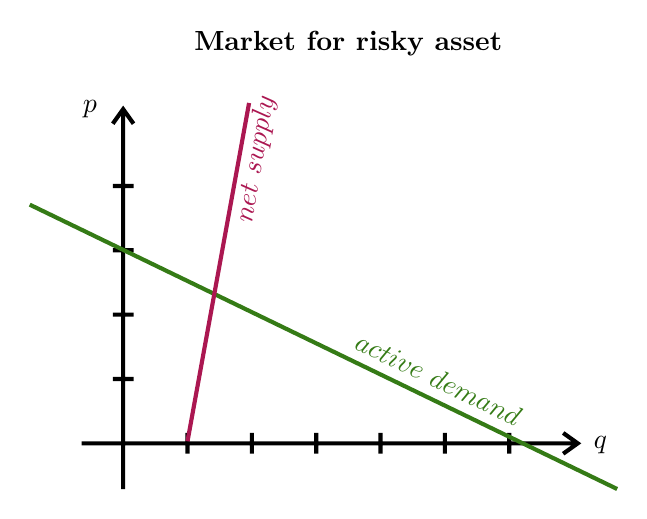
\begin{tikzpicture}[x=0.75pt,y=0.75pt,yscale=-1,xscale=1]
	%uncomment if require: \path (0,235); %set diagram left start at 0, and has height of 235
	
	%Shape: Axis 2D [id:dp3699485075380834] 
	\draw [color={rgb, 255:red, 0; green, 0; blue, 0 }  ,draw opacity=1 ][line width=1.5]  (380,200) -- (619,200)(400,39) -- (400,222) (612,195) -- (619,200) -- (612,205) (395,46) -- (400,39) -- (405,46) (431,195) -- (431,205)(462,195) -- (462,205)(493,195) -- (493,205)(524,195) -- (524,205)(555,195) -- (555,205)(586,195) -- (586,205)(395,169) -- (405,169)(395,138) -- (405,138)(395,107) -- (405,107)(395,76) -- (405,76) ;
	\draw   ;
	%Straight Lines [id:da7483554761171687] 
	\draw [color={rgb, 255:red, 65; green, 117; blue, 5 }  ,draw opacity=1 ][line width=1.5]    (355,85) -- (638,222) ;
	%Straight Lines [id:da38811786243247126] 
	\draw [color={rgb, 255:red, 208; green, 2; blue, 27 }  ,draw opacity=1 ][line width=1.5]    (431,199) -- (460.67,36) ;
	
	% Text Node
	\draw (464,63) node  [color={rgb, 255:red, 208; green, 2; blue, 27 }  ,opacity=1 ,rotate=-279.88]  {$net\ supply$};
	% Text Node
	\draw (630,201) node  [color={rgb, 255:red, 0; green, 0; blue, 0 }  ,opacity=1 ,rotate=-358.98]  {$q$};
	% Text Node
	\draw (552,169) node  [color={rgb, 255:red, 65; green, 117; blue, 5 }  ,opacity=1 ,rotate=-25.74]  {$active\ demand$};
	% Text Node
	\draw (384,39) node  [color={rgb, 255:red, 0; green, 0; blue, 0 }  ,opacity=1 ,rotate=-358.98]  {$p$};
	% Text Node
	\draw (433,0) node [anchor=north west][inner sep=0.75pt]   [align=left] {\textbf{Market for risky asset}};
	
	
\end{tikzpicture}
	\end{column}
\end{columns}
\end{frame}

\begin{frame}{The market for goods}
\begin{columns}
	\begin{column}{0.55\textwidth}			
\tikzset{every picture/.style={line width=0.75pt}} %set default line width to 0.75pt        

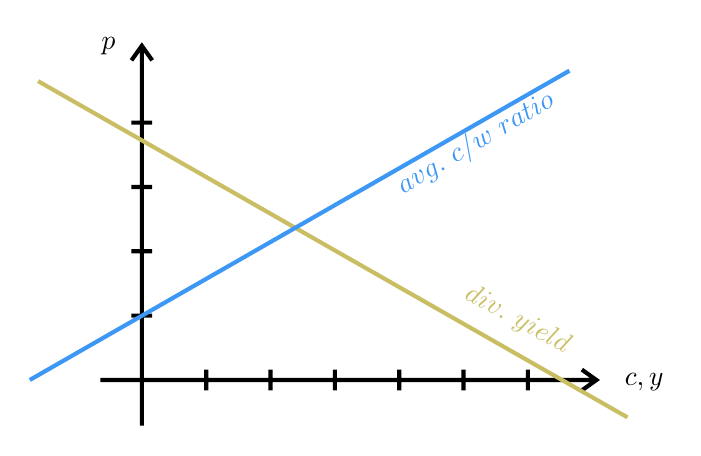
\begin{tikzpicture}[x=0.75pt,y=0.75pt,yscale=-1,xscale=1]
	%uncomment if require: \path (0,235); %set diagram left start at 0, and has height of 235
	
	%Shape: Axis 2D [id:dp5132950601646007] 
	\draw [color={rgb, 255:red, 0; green, 0; blue, 0 }  ,draw opacity=1 ][line width=1.5]  (50,200) -- (289,200)(70,39) -- (70,222) (282,195) -- (289,200) -- (282,205) (65,46) -- (70,39) -- (75,46) (101,195) -- (101,205)(132,195) -- (132,205)(163,195) -- (163,205)(194,195) -- (194,205)(225,195) -- (225,205)(256,195) -- (256,205)(65,169) -- (75,169)(65,138) -- (75,138)(65,107) -- (75,107)(65,76) -- (75,76) ;
	\draw   ;
	%Straight Lines [id:da929233454246288] 
	\draw [color={rgb, 255:red, 245; green, 166; blue, 35 }  ,draw opacity=1 ][line width=1.5]    (20,56) -- (304,218) ;
	%Straight Lines [id:da5921961944005785] 
	\draw [color={rgb, 255:red, 74; green, 144; blue, 226 }  ,draw opacity=1 ][line width=1.5]    (16,200) -- (276,51) ;
	
	% Text Node
	\draw (231,86) node  [color={rgb, 255:red, 74; green, 144; blue, 226 }  ,opacity=1 ,rotate=-329.57]  {$avg.\ c/w\ ratio$};
	% Text Node
	\draw (312,201) node  [color={rgb, 255:red, 0; green, 0; blue, 0 }  ,opacity=1 ,rotate=-358.98]  {$c,y$};
	% Text Node
	\draw (251,171) node  [color={rgb, 255:red, 245; green, 166; blue, 35 }  ,opacity=1 ,rotate=-28.61]  {$div.\ yield$};
	% Text Node
	\draw (54,39) node  [color={rgb, 255:red, 0; green, 0; blue, 0 }  ,opacity=1 ,rotate=-358.98]  {$p$};
	
	
\end{tikzpicture}
	\end{column}
	\begin{column}{0.45\textwidth}  %%<--- here
		\textcolor{blue}{Goods mkt. clearing:} 
		\[
		\underbrace{\sum_{j\in\{p,a\}} x_j c_j(\mu-p) }_{\textbf{consumption-wealth ratio}}  = \underbrace{\frac{1}{1+e^p}}_{\textbf{dividend yield}},
		\]\small
		given type-$j$ wealth share  $x_j$.
	\end{column}
\end{columns}
\end{frame}

\begin{frame}{Equilibrium}



\tikzset{every picture/.style={line width=0.75pt}} %set default line width to 0.75pt        
\scalebox{0.9}{
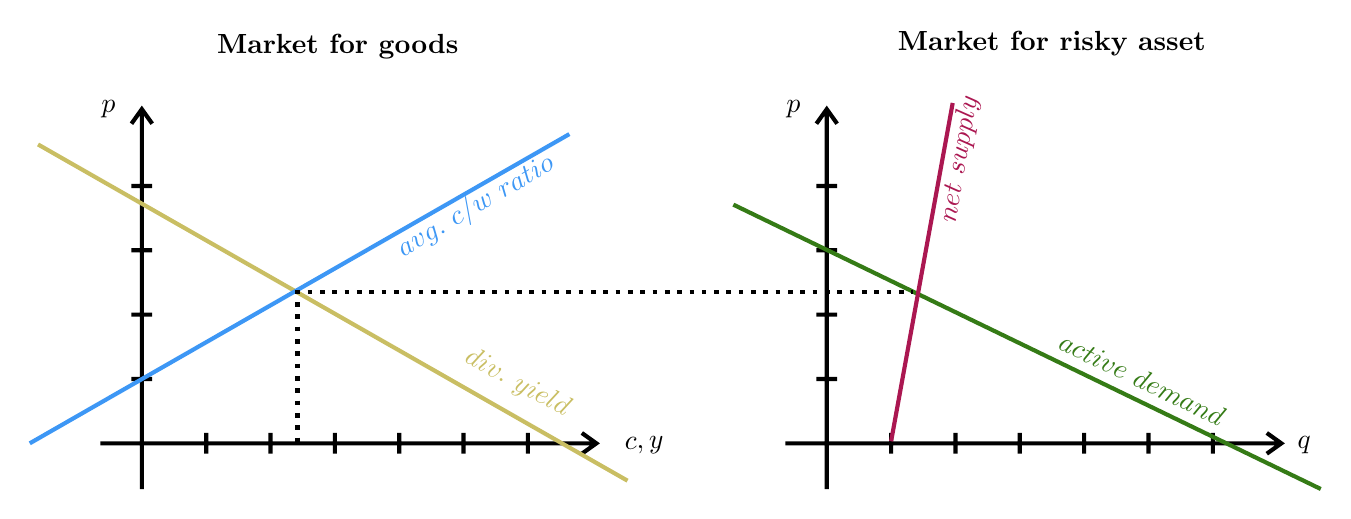
\begin{tikzpicture}[x=0.75pt,y=0.75pt,yscale=-1,xscale=1]
	%uncomment if require: \path (0,235); %set diagram left start at 0, and has height of 235
	
	%Shape: Axis 2D [id:dp5132950601646007] 
	\draw [color={rgb, 255:red, 0; green, 0; blue, 0 }  ,draw opacity=1 ][line width=1.5]  (50,200) -- (289,200)(70,39) -- (70,222) (282,195) -- (289,200) -- (282,205) (65,46) -- (70,39) -- (75,46) (101,195) -- (101,205)(132,195) -- (132,205)(163,195) -- (163,205)(194,195) -- (194,205)(225,195) -- (225,205)(256,195) -- (256,205)(65,169) -- (75,169)(65,138) -- (75,138)(65,107) -- (75,107)(65,76) -- (75,76) ;
	\draw   ;
	%Straight Lines [id:da929233454246288] 
	\draw [color={rgb, 255:red, 245; green, 166; blue, 35 }  ,draw opacity=1 ][line width=1.5]    (20,56) -- (304,218) ;
	%Straight Lines [id:da5921961944005785] 
	\draw [color={rgb, 255:red, 74; green, 144; blue, 226 }  ,draw opacity=1 ][line width=1.5]    (16,200) -- (276,51) ;
	%Straight Lines [id:da2953578261472096] 
	\draw [color={rgb, 255:red, 0; green, 0; blue, 0 }  ,draw opacity=1 ][line width=1.5]  [dash pattern={on 1.69pt off 2.76pt}]  (145,126) -- (145,200) ;
	%Shape: Axis 2D [id:dp3699485075380834] 
	\draw [color={rgb, 255:red, 0; green, 0; blue, 0 }  ,draw opacity=1 ][line width=1.5]  (380,200) -- (619,200)(400,39) -- (400,222) (612,195) -- (619,200) -- (612,205) (395,46) -- (400,39) -- (405,46) (431,195) -- (431,205)(462,195) -- (462,205)(493,195) -- (493,205)(524,195) -- (524,205)(555,195) -- (555,205)(586,195) -- (586,205)(395,169) -- (405,169)(395,138) -- (405,138)(395,107) -- (405,107)(395,76) -- (405,76) ;
	\draw   ;
	%Straight Lines [id:da7483554761171687] 
	\draw [color={rgb, 255:red, 65; green, 117; blue, 5 }  ,draw opacity=1 ][line width=1.5]    (355,85) -- (638,222) ;
	%Straight Lines [id:da38811786243247126] 
	\draw [color={rgb, 255:red, 208; green, 2; blue, 27 }  ,draw opacity=1 ][line width=1.5]    (431,199) -- (460.67,36) ;
	%Straight Lines [id:da4060861160692876] 
	\draw [color={rgb, 255:red, 0; green, 0; blue, 0 }  ,draw opacity=1 ][line width=1.5]  [dash pattern={on 1.69pt off 2.76pt}]  (144,127) -- (441.4,127) ;
	
	% Text Node
	\draw (231,86) node  [color={rgb, 255:red, 74; green, 144; blue, 226 }  ,opacity=1 ,rotate=-329.57]  {$avg.\ c/w\ ratio$};
	% Text Node
	\draw (312,201) node  [color={rgb, 255:red, 0; green, 0; blue, 0 }  ,opacity=1 ,rotate=-358.98]  {$c,y$};
	% Text Node
	\draw (251,171) node  [color={rgb, 255:red, 245; green, 166; blue, 35 }  ,opacity=1 ,rotate=-28.61]  {$div.\ yield$};
	% Text Node
	\draw (54,39) node  [color={rgb, 255:red, 0; green, 0; blue, 0 }  ,opacity=1 ,rotate=-358.98]  {$p$};
	% Text Node
	\draw (464,63) node  [color={rgb, 255:red, 208; green, 2; blue, 27 }  ,opacity=1 ,rotate=-279.88]  {$net\ supply$};
	% Text Node
	\draw (630,201) node  [color={rgb, 255:red, 0; green, 0; blue, 0 }  ,opacity=1 ,rotate=-358.98]  {$q$};
	% Text Node
	\draw (552,169) node  [color={rgb, 255:red, 65; green, 117; blue, 5 }  ,opacity=1 ,rotate=-25.74]  {$active\ demand$};
	% Text Node
	\draw (384,39) node  [color={rgb, 255:red, 0; green, 0; blue, 0 }  ,opacity=1 ,rotate=-358.98]  {$p$};
	% Text Node
	\draw (105,1.43) node [anchor=north west][inner sep=0.75pt]   [align=left] {\textbf{Market for goods}};
	% Text Node
	\draw (433,0) node [anchor=north west][inner sep=0.75pt]   [align=left] {\textbf{Market for risky asset}};
	
	
\end{tikzpicture}}
\end{frame}


\begin{frame}{Introducing portfolio flow shocks}

\textcolor{blue}{A portfolio flow shock:}
\begin{itemize}
	\item Reference economy: passive port. share $\overline{\alpha}_p^*$ and prices $(p^*,r^*)$
	\item Economy of interest: $\overline{\alpha}_p = \overline{\alpha}_p^* e^{\hat{\alpha}_p}$, where $\hat{\alpha}_p$ is small
\begin{itemize}
		\item What is the impact of changes in $\hat{\alpha}_p$?
		\item Positive $\hat{\alpha}_p$ means flow of funds from riskless to risky asset
\end{itemize}
\end{itemize} 

\vspH \pause

\textcolor{blue}{Demand for the risky asset:}
\begin{itemize}
	\item Let $q_j \equiv \log Q_j / Q_j^*$, then
	\[ q_j = \zeta_{j,0}^q - \textcolor{darkred}{\zeta_{j,p}^q} p - \textcolor{darkblue}{\zeta_{j,r}^q} r + \textcolor{darkgreen}{f_{j}} \],
\end{itemize} \small
where $ \textcolor{darkred}{\zeta_{j,p}^q} = - \frac{\partial \log Q_j}{\partial p}$, 
$ \textcolor{darkblue}{\zeta_{j,r}^q} = - \frac{\partial \log Q_j}{\partial r}$, and $\textcolor{darkgreen}{f_{j}} =  \frac{\partial \log Q_j}{\partial \overline{\alpha}_p} \hat{\alpha}_p $.
\end{frame}


\begin{frame}{The demand system}
	
	\textcolor{blue}{The goods market:}
	\begin{itemize}
		\item Linearizing the goods market clearing condition:
		\[ \zeta_p^c(p - p^*) = - \frac{e^{p^*}}{(1+e^{p^*})^2} (p-p^*),\]
		where $\zeta^c_p = - c'(\mu - p)$.
	\end{itemize} 

\vspH

	\textcolor{blue}{The demand system:}
	\[
	\left[ 
	\begin{matrix}
		\zeta_p^q & \zeta_r^q \\
		\zeta_p^c + \frac{e^{p^*}}{(1+e^{p^*})^2} & 0
	\end{matrix}
	\right] \left[ 
	\begin{matrix}
		p-p^*\\
		r-r^*
	\end{matrix}
	\right] = 
	\left[ 
	\begin{matrix}
		f\\
		0
		\end{matrix}
	\right].
	\]
\end{frame}

\begin{frame}{The inelastic market hypothesis}
	
	\begin{columns}
		\begin{column}{0.45\textwidth}			

\textcolor{blue}{A partial equilibrium exercise:}
\begin{itemize}
	\item Suppose $r$ is fixed or $\zeta^p_r = 0$
		\item As in Gabaix and Koijen (2020)
	\item The price impact is given by
\end{itemize} 
\[
  p - p^* = \textcolor{darkblue}{ \underbrace{\frac{1}{\zeta_p^q}}_{\substack{\textbf{inverse mkt.}\\ \textbf{elasticity}}}} \times 
  \textcolor{darkred}{  \underbrace{f}_{\textbf{flow shock}}},
\]\small
where $\zeta_p^q = \sum_{j\in\{p,a\}} x_j \zeta_{j,p}^q $.
		\end{column}
		\begin{column}{0.55\textwidth}  %%<--- here
			\tikzset{every picture/.style={line width=0.75pt}} %set default line width to 0.75pt        
			
			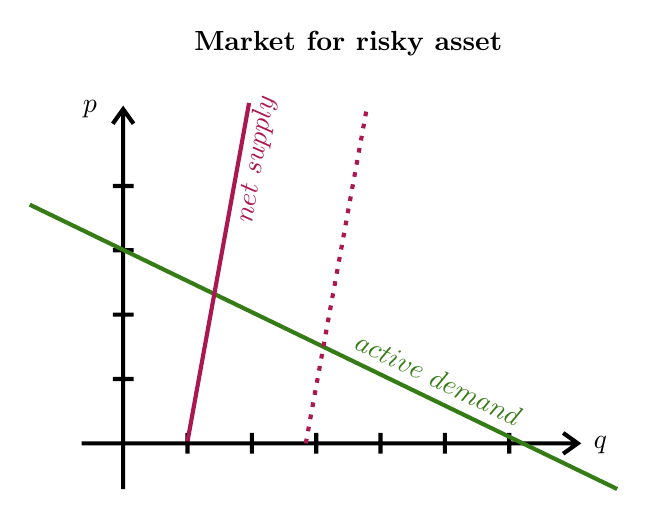
\begin{tikzpicture}[x=0.75pt,y=0.75pt,yscale=-1,xscale=1]
				%uncomment if require: \path (0,235); %set diagram left start at 0, and has height of 235
				
				%Shape: Axis 2D [id:dp3699485075380834] 
				\draw [color={rgb, 255:red, 0; green, 0; blue, 0 }  ,draw opacity=1 ][line width=1.5]  (380,200) -- (619,200)(400,39) -- (400,222) (612,195) -- (619,200) -- (612,205) (395,46) -- (400,39) -- (405,46) (431,195) -- (431,205)(462,195) -- (462,205)(493,195) -- (493,205)(524,195) -- (524,205)(555,195) -- (555,205)(586,195) -- (586,205)(395,169) -- (405,169)(395,138) -- (405,138)(395,107) -- (405,107)(395,76) -- (405,76) ;
				\draw   ;
				%Straight Lines [id:da7483554761171687] 
				\draw [color={rgb, 255:red, 65; green, 117; blue, 5 }  ,draw opacity=1 ][line width=1.5]    (355,85) -- (638,222) ;
				%Straight Lines [id:da38811786243247126] 
				\draw [color={rgb, 255:red, 208; green, 2; blue, 27 }  ,draw opacity=1 ][line width=1.5]    (431,199) -- (460.67,36) ;
				%Straight Lines [id:da21438260220121663] 
				\draw [color={rgb, 255:red, 208; green, 2; blue, 27 }  ,draw opacity=1 ][line width=1.5]  [dash pattern={on 1.69pt off 2.76pt}]  (488,200) -- (517.67,37) ;
				
				% Text Node
				\draw (464,63) node  [color={rgb, 255:red, 208; green, 2; blue, 27 }  ,opacity=1 ,rotate=-279.88]  {$net\ supply$};
				% Text Node
				\draw (630,201) node  [color={rgb, 255:red, 0; green, 0; blue, 0 }  ,opacity=1 ,rotate=-358.98]  {$q$};
				% Text Node
				\draw (552,169) node  [color={rgb, 255:red, 65; green, 117; blue, 5 }  ,opacity=1 ,rotate=-25.74]  {$active\ demand$};
				% Text Node
				\draw (384,39) node  [color={rgb, 255:red, 0; green, 0; blue, 0 }  ,opacity=1 ,rotate=-358.98]  {$p$};
				% Text Node
				\draw (433,0) node [anchor=north west][inner sep=0.75pt]   [align=left] {\textbf{Market for risky asset}};
				
				
			\end{tikzpicture}
		\end{column}
	\end{columns}
	
\end{frame}

\begin{frame}{The importance of cross-elasticity}
\only<1>{ \scalebox{0.85}{
	
	
	\tikzset{every picture/.style={line width=0.75pt}} %set default line width to 0.75pt        
	
	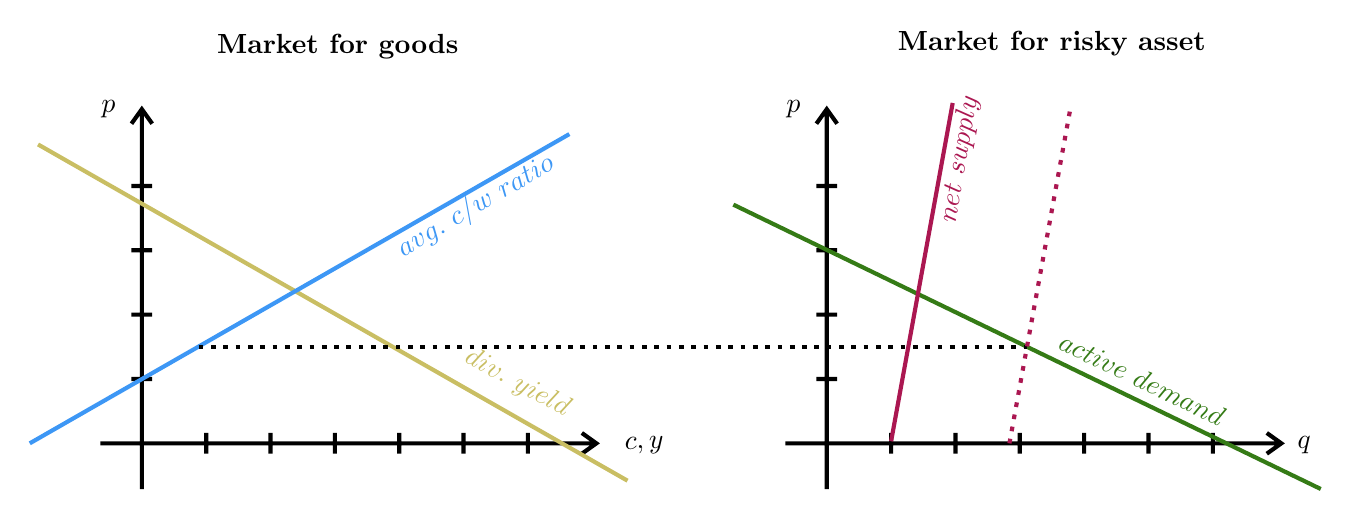
\begin{tikzpicture}[x=0.75pt,y=0.75pt,yscale=-1,xscale=1]
		%uncomment if require: \path (0,235); %set diagram left start at 0, and has height of 235
		
		%Shape: Axis 2D [id:dp5132950601646007] 
		\draw [color={rgb, 255:red, 0; green, 0; blue, 0 }  ,draw opacity=1 ][line width=1.5]  (50,200) -- (289,200)(70,39) -- (70,222) (282,195) -- (289,200) -- (282,205) (65,46) -- (70,39) -- (75,46) (101,195) -- (101,205)(132,195) -- (132,205)(163,195) -- (163,205)(194,195) -- (194,205)(225,195) -- (225,205)(256,195) -- (256,205)(65,169) -- (75,169)(65,138) -- (75,138)(65,107) -- (75,107)(65,76) -- (75,76) ;
		\draw   ;
		%Straight Lines [id:da929233454246288] 
		\draw [color={rgb, 255:red, 245; green, 166; blue, 35 }  ,draw opacity=1 ][line width=1.5]    (20,56) -- (304,218) ;
		%Straight Lines [id:da5921961944005785] 
		\draw [color={rgb, 255:red, 74; green, 144; blue, 226 }  ,draw opacity=1 ][line width=1.5]    (16,200) -- (276,51) ;
		%Shape: Axis 2D [id:dp3699485075380834] 
		\draw [color={rgb, 255:red, 0; green, 0; blue, 0 }  ,draw opacity=1 ][line width=1.5]  (380,200) -- (619,200)(400,39) -- (400,222) (612,195) -- (619,200) -- (612,205) (395,46) -- (400,39) -- (405,46) (431,195) -- (431,205)(462,195) -- (462,205)(493,195) -- (493,205)(524,195) -- (524,205)(555,195) -- (555,205)(586,195) -- (586,205)(395,169) -- (405,169)(395,138) -- (405,138)(395,107) -- (405,107)(395,76) -- (405,76) ;
		\draw   ;
		%Straight Lines [id:da7483554761171687] 
		\draw [color={rgb, 255:red, 65; green, 117; blue, 5 }  ,draw opacity=1 ][line width=1.5]    (355,85) -- (638,222) ;
		%Straight Lines [id:da38811786243247126] 
		\draw [color={rgb, 255:red, 208; green, 2; blue, 27 }  ,draw opacity=1 ][line width=1.5]    (431,199) -- (460.67,36) ;
		%Straight Lines [id:da4060861160692876] 
		\draw [color={rgb, 255:red, 0; green, 0; blue, 0 }  ,draw opacity=1 ][line width=1.5]  [dash pattern={on 1.69pt off 2.76pt}]  (97.4,153.5) -- (496.5,153.5) ;
		%Straight Lines [id:da21438260220121663] 
		\draw [color={rgb, 255:red, 208; green, 2; blue, 27 }  ,draw opacity=1 ][line width=1.5]  [dash pattern={on 1.69pt off 2.76pt}]  (488,200) -- (517.67,37) ;
		
		% Text Node
		\draw (231,86) node  [color={rgb, 255:red, 74; green, 144; blue, 226 }  ,opacity=1 ,rotate=-329.57]  {$avg.\ c/w\ ratio$};
		% Text Node
		\draw (312,201) node  [color={rgb, 255:red, 0; green, 0; blue, 0 }  ,opacity=1 ,rotate=-358.98]  {$c,y$};
		% Text Node
		\draw (251,171) node  [color={rgb, 255:red, 245; green, 166; blue, 35 }  ,opacity=1 ,rotate=-28.61]  {$div.\ yield$};
		% Text Node
		\draw (54,39) node  [color={rgb, 255:red, 0; green, 0; blue, 0 }  ,opacity=1 ,rotate=-358.98]  {$p$};
		% Text Node
		\draw (464,63) node  [color={rgb, 255:red, 208; green, 2; blue, 27 }  ,opacity=1 ,rotate=-279.88]  {$net\ supply$};
		% Text Node
		\draw (630,201) node  [color={rgb, 255:red, 0; green, 0; blue, 0 }  ,opacity=1 ,rotate=-358.98]  {$q$};
		% Text Node
		\draw (552,169) node  [color={rgb, 255:red, 65; green, 117; blue, 5 }  ,opacity=1 ,rotate=-25.74]  {$active\ demand$};
		% Text Node
		\draw (384,39) node  [color={rgb, 255:red, 0; green, 0; blue, 0 }  ,opacity=1 ,rotate=-358.98]  {$p$};
		% Text Node
		\draw (105,1.43) node [anchor=north west][inner sep=0.75pt]   [align=left] {\textbf{Market for goods}};
		% Text Node
		\draw (433,0) node [anchor=north west][inner sep=0.75pt]   [align=left] {\textbf{Market for risky asset}};
		
		
\end{tikzpicture}}}\pause
\only<2>{
\scalebox{0.85}{



\tikzset{every picture/.style={line width=0.75pt}} %set default line width to 0.75pt        

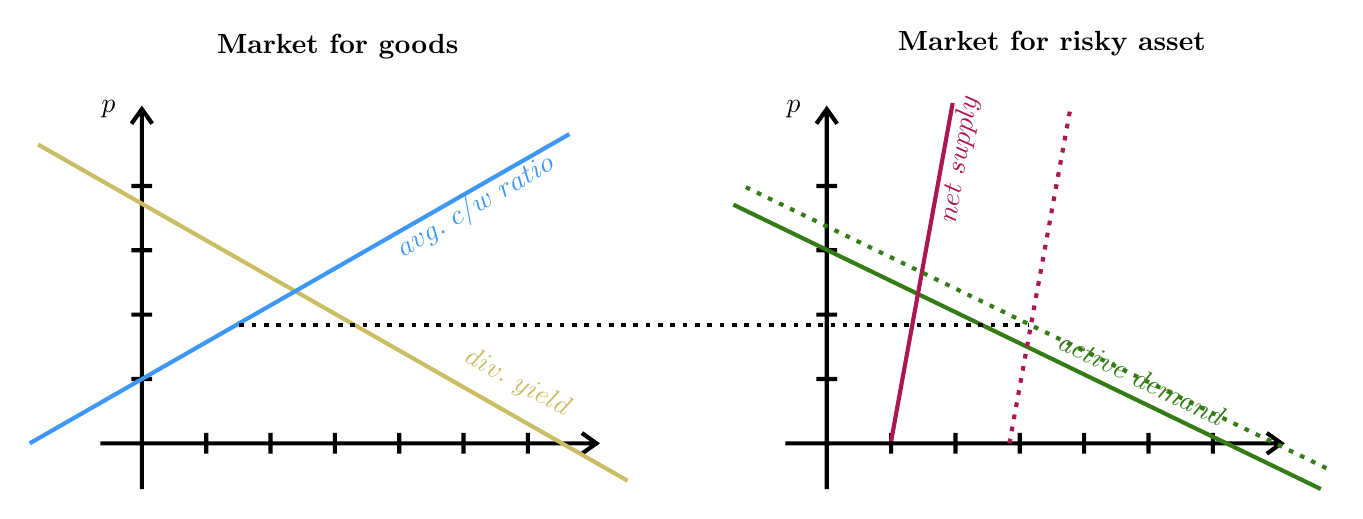
\begin{tikzpicture}[x=0.75pt,y=0.75pt,yscale=-1,xscale=1]
	%uncomment if require: \path (0,235); %set diagram left start at 0, and has height of 235
	
	%Shape: Axis 2D [id:dp5132950601646007] 
	\draw [color={rgb, 255:red, 0; green, 0; blue, 0 }  ,draw opacity=1 ][line width=1.5]  (50,200) -- (289,200)(70,39) -- (70,222) (282,195) -- (289,200) -- (282,205) (65,46) -- (70,39) -- (75,46) (101,195) -- (101,205)(132,195) -- (132,205)(163,195) -- (163,205)(194,195) -- (194,205)(225,195) -- (225,205)(256,195) -- (256,205)(65,169) -- (75,169)(65,138) -- (75,138)(65,107) -- (75,107)(65,76) -- (75,76) ;
	\draw   ;
	%Straight Lines [id:da929233454246288] 
	\draw [color={rgb, 255:red, 245; green, 166; blue, 35 }  ,draw opacity=1 ][line width=1.5]    (20,56) -- (304,218) ;
	%Straight Lines [id:da5921961944005785] 
	\draw [color={rgb, 255:red, 74; green, 144; blue, 226 }  ,draw opacity=1 ][line width=1.5]    (16,200) -- (276,51) ;
	%Shape: Axis 2D [id:dp3699485075380834] 
	\draw [color={rgb, 255:red, 0; green, 0; blue, 0 }  ,draw opacity=1 ][line width=1.5]  (380,200) -- (619,200)(400,39) -- (400,222) (612,195) -- (619,200) -- (612,205) (395,46) -- (400,39) -- (405,46) (431,195) -- (431,205)(462,195) -- (462,205)(493,195) -- (493,205)(524,195) -- (524,205)(555,195) -- (555,205)(586,195) -- (586,205)(395,169) -- (405,169)(395,138) -- (405,138)(395,107) -- (405,107)(395,76) -- (405,76) ;
	\draw   ;
	%Straight Lines [id:da7483554761171687] 
	\draw [color={rgb, 255:red, 65; green, 117; blue, 5 }  ,draw opacity=1 ][line width=1.5]    (355,85) -- (638,222) ;
	%Straight Lines [id:da38811786243247126] 
	\draw [color={rgb, 255:red, 208; green, 2; blue, 27 }  ,draw opacity=1 ][line width=1.5]    (431,199) -- (460.67,36) ;
	%Straight Lines [id:da4060861160692876] 
	\draw [color={rgb, 255:red, 0; green, 0; blue, 0 }  ,draw opacity=1 ][line width=1.5]  [dash pattern={on 1.69pt off 2.76pt}]  (117,143) -- (497.4,143) ;
	%Straight Lines [id:da3647922931527937] 
	\draw [color={rgb, 255:red, 65; green, 117; blue, 5 }  ,draw opacity=1 ][line width=1.5]  [dash pattern={on 1.69pt off 2.76pt}]  (361,76.57) -- (644,213.57) ;
	%Straight Lines [id:da21438260220121663] 
	\draw [color={rgb, 255:red, 208; green, 2; blue, 27 }  ,draw opacity=1 ][line width=1.5]  [dash pattern={on 1.69pt off 2.76pt}]  (488,200) -- (517.67,37) ;
	
	% Text Node
	\draw (231,86) node  [color={rgb, 255:red, 74; green, 144; blue, 226 }  ,opacity=1 ,rotate=-329.57]  {$avg.\ c/w\ ratio$};
	% Text Node
	\draw (251,171) node  [color={rgb, 255:red, 245; green, 166; blue, 35 }  ,opacity=1 ,rotate=-28.61]  {$div.\ yield$};
	% Text Node
	\draw (54,39) node  [color={rgb, 255:red, 0; green, 0; blue, 0 }  ,opacity=1 ,rotate=-358.98]  {$p$};
	% Text Node
	\draw (464,63) node  [color={rgb, 255:red, 208; green, 2; blue, 27 }  ,opacity=1 ,rotate=-279.88]  {$net\ supply$};
	% Text Node
	\draw (552,169) node  [color={rgb, 255:red, 65; green, 117; blue, 5 }  ,opacity=1 ,rotate=-25.74]  {$active\ demand$};
	% Text Node
	\draw (384,39) node  [color={rgb, 255:red, 0; green, 0; blue, 0 }  ,opacity=1 ,rotate=-358.98]  {$p$};
	% Text Node
	\draw (105,1.43) node [anchor=north west][inner sep=0.75pt]   [align=left] {\textbf{Market for goods}};
	% Text Node
	\draw (433,0) node [anchor=north west][inner sep=0.75pt]   [align=left] {\textbf{Market for risky asset}};
	
	
\end{tikzpicture}
}
}\pause
\only<3>{
\scalebox{0.85}{



\tikzset{every picture/.style={line width=0.75pt}} %set default line width to 0.75pt        

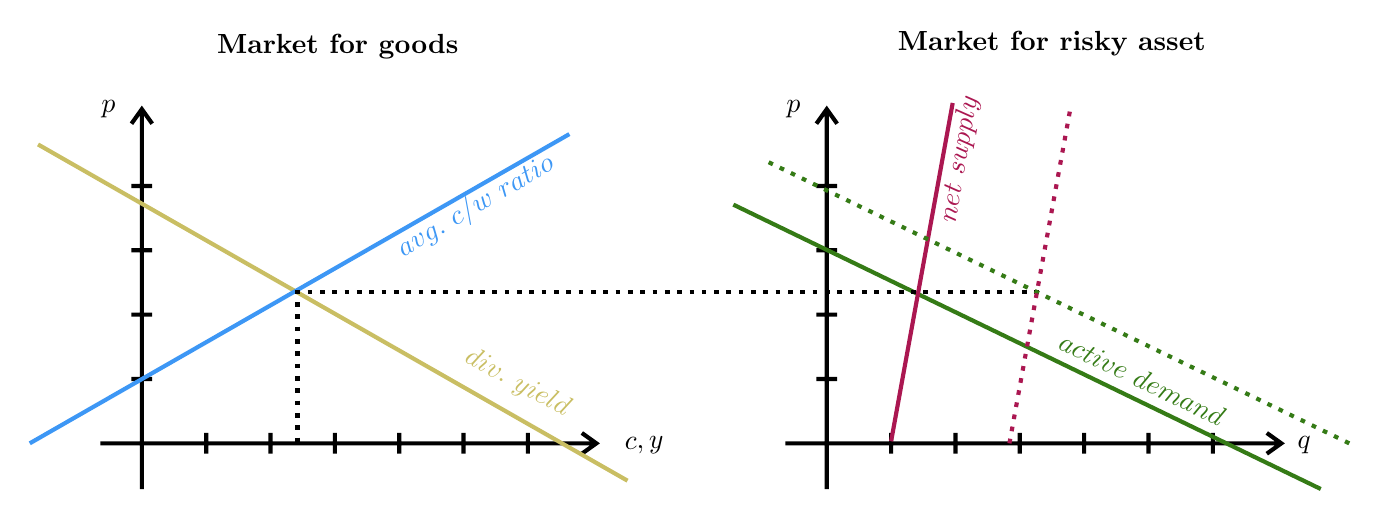
\begin{tikzpicture}[x=0.75pt,y=0.75pt,yscale=-1,xscale=1]
	%uncomment if require: \path (0,235); %set diagram left start at 0, and has height of 235
	
	%Shape: Axis 2D [id:dp5132950601646007] 
	\draw [color={rgb, 255:red, 0; green, 0; blue, 0 }  ,draw opacity=1 ][line width=1.5]  (50,200) -- (289,200)(70,39) -- (70,222) (282,195) -- (289,200) -- (282,205) (65,46) -- (70,39) -- (75,46) (101,195) -- (101,205)(132,195) -- (132,205)(163,195) -- (163,205)(194,195) -- (194,205)(225,195) -- (225,205)(256,195) -- (256,205)(65,169) -- (75,169)(65,138) -- (75,138)(65,107) -- (75,107)(65,76) -- (75,76) ;
	\draw   ;
	%Straight Lines [id:da929233454246288] 
	\draw [color={rgb, 255:red, 245; green, 166; blue, 35 }  ,draw opacity=1 ][line width=1.5]    (20,56) -- (304,218) ;
	%Straight Lines [id:da5921961944005785] 
	\draw [color={rgb, 255:red, 74; green, 144; blue, 226 }  ,draw opacity=1 ][line width=1.5]    (16,200) -- (276,51) ;
	%Straight Lines [id:da2953578261472096] 
	\draw [color={rgb, 255:red, 0; green, 0; blue, 0 }  ,draw opacity=1 ][line width=1.5]  [dash pattern={on 1.69pt off 2.76pt}]  (145,126) -- (145,200) ;
	%Shape: Axis 2D [id:dp3699485075380834] 
	\draw [color={rgb, 255:red, 0; green, 0; blue, 0 }  ,draw opacity=1 ][line width=1.5]  (380,200) -- (619,200)(400,39) -- (400,222) (612,195) -- (619,200) -- (612,205) (395,46) -- (400,39) -- (405,46) (431,195) -- (431,205)(462,195) -- (462,205)(493,195) -- (493,205)(524,195) -- (524,205)(555,195) -- (555,205)(586,195) -- (586,205)(395,169) -- (405,169)(395,138) -- (405,138)(395,107) -- (405,107)(395,76) -- (405,76) ;
	\draw   ;
	%Straight Lines [id:da7483554761171687] 
	\draw [color={rgb, 255:red, 65; green, 117; blue, 5 }  ,draw opacity=1 ][line width=1.5]    (355,85) -- (638,222) ;
	%Straight Lines [id:da38811786243247126] 
	\draw [color={rgb, 255:red, 208; green, 2; blue, 27 }  ,draw opacity=1 ][line width=1.5]    (431,199) -- (460.67,36) ;
	%Straight Lines [id:da4060861160692876] 
	\draw [color={rgb, 255:red, 0; green, 0; blue, 0 }  ,draw opacity=1 ][line width=1.5]  [dash pattern={on 1.69pt off 2.76pt}]  (144,127) -- (504.67,127) ;
	%Straight Lines [id:da3647922931527937] 
	\draw [color={rgb, 255:red, 65; green, 117; blue, 5 }  ,draw opacity=1 ][line width=1.5]  [dash pattern={on 1.69pt off 2.76pt}]  (372,64.57) -- (655,201.57) ;
	%Straight Lines [id:da21438260220121663] 
	\draw [color={rgb, 255:red, 208; green, 2; blue, 27 }  ,draw opacity=1 ][line width=1.5]  [dash pattern={on 1.69pt off 2.76pt}]  (488,200) -- (517.67,37) ;
	
	% Text Node
	\draw (231,86) node  [color={rgb, 255:red, 74; green, 144; blue, 226 }  ,opacity=1 ,rotate=-329.57]  {$avg.\ c/w\ ratio$};
	% Text Node
	\draw (312,201) node  [color={rgb, 255:red, 0; green, 0; blue, 0 }  ,opacity=1 ,rotate=-358.98]  {$c,y$};
	% Text Node
	\draw (251,171) node  [color={rgb, 255:red, 245; green, 166; blue, 35 }  ,opacity=1 ,rotate=-28.61]  {$div.\ yield$};
	% Text Node
	\draw (54,39) node  [color={rgb, 255:red, 0; green, 0; blue, 0 }  ,opacity=1 ,rotate=-358.98]  {$p$};
	% Text Node
	\draw (464,63) node  [color={rgb, 255:red, 208; green, 2; blue, 27 }  ,opacity=1 ,rotate=-279.88]  {$net\ supply$};
	% Text Node
	\draw (630,201) node  [color={rgb, 255:red, 0; green, 0; blue, 0 }  ,opacity=1 ,rotate=-358.98]  {$q$};
	% Text Node
	\draw (552,169) node  [color={rgb, 255:red, 65; green, 117; blue, 5 }  ,opacity=1 ,rotate=-25.74]  {$active\ demand$};
	% Text Node
	\draw (384,39) node  [color={rgb, 255:red, 0; green, 0; blue, 0 }  ,opacity=1 ,rotate=-358.98]  {$p$};
	% Text Node
	\draw (105,1.43) node [anchor=north west][inner sep=0.75pt]   [align=left] {\textbf{Market for goods}};
	% Text Node
	\draw (433,0) node [anchor=north west][inner sep=0.75pt]   [align=left] {\textbf{Market for risky asset}};
	
	
\end{tikzpicture}
}
}

\visible<3>{
\textcolor{blue}{Market is infinitely elastic:}
\begin{itemize}
	\item \textcolor{red}{\textbf{Price impact is zero}:} $p - p^* = 0$
	\item This holds regardless of how inelastic individual investors are
\end{itemize} 
}

\end{frame}

\begin{frame}{A finite aggregate elasticity in GE}

\textcolor{blue}{When is the aggregate market elasticity finite?}
\begin{itemize}
	\item Consider the following variation of the basic model: $c(r+\pi, \overline{\alpha_p}$)
	\item Portfolio flows affects consumption/savings decision directly
\end{itemize} \pause
	
\scalebox{0.85}{
	
	
	\tikzset{every picture/.style={line width=0.75pt}} %set default line width to 0.75pt        
	
	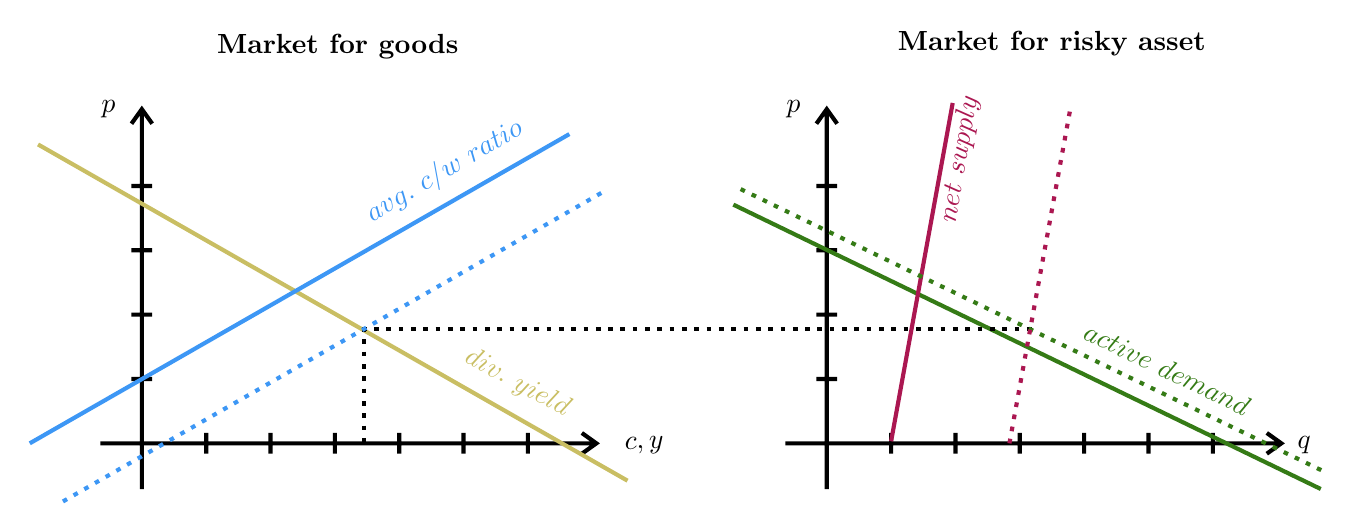
\begin{tikzpicture}[x=0.75pt,y=0.75pt,yscale=-1,xscale=1]
		%uncomment if require: \path (0,235); %set diagram left start at 0, and has height of 235
		
		%Shape: Axis 2D [id:dp05601326687806596] 
		\draw [color={rgb, 255:red, 0; green, 0; blue, 0 }  ,draw opacity=1 ][line width=1.5]  (50,200) -- (289,200)(70,39) -- (70,222) (282,195) -- (289,200) -- (282,205) (65,46) -- (70,39) -- (75,46) (101,195) -- (101,205)(132,195) -- (132,205)(163,195) -- (163,205)(194,195) -- (194,205)(225,195) -- (225,205)(256,195) -- (256,205)(65,169) -- (75,169)(65,138) -- (75,138)(65,107) -- (75,107)(65,76) -- (75,76) ;
		\draw   ;
		%Straight Lines [id:da30482939986645063] 
		\draw [color={rgb, 255:red, 245; green, 166; blue, 35 }  ,draw opacity=1 ][line width=1.5]    (20,56) -- (304,218) ;
		%Straight Lines [id:da8049359477241715] 
		\draw [color={rgb, 255:red, 74; green, 144; blue, 226 }  ,draw opacity=1 ][line width=1.5]    (16,200) -- (276,51) ;
		%Straight Lines [id:da3248253140368892] 
		\draw [color={rgb, 255:red, 0; green, 0; blue, 0 }  ,draw opacity=1 ][line width=1.5]  [dash pattern={on 1.69pt off 2.76pt}]  (177,144) -- (177,201) ;
		%Shape: Axis 2D [id:dp4494371234769491] 
		\draw [color={rgb, 255:red, 0; green, 0; blue, 0 }  ,draw opacity=1 ][line width=1.5]  (380,200) -- (619,200)(400,39) -- (400,222) (612,195) -- (619,200) -- (612,205) (395,46) -- (400,39) -- (405,46) (431,195) -- (431,205)(462,195) -- (462,205)(493,195) -- (493,205)(524,195) -- (524,205)(555,195) -- (555,205)(586,195) -- (586,205)(395,169) -- (405,169)(395,138) -- (405,138)(395,107) -- (405,107)(395,76) -- (405,76) ;
		\draw   ;
		%Straight Lines [id:da5121385722918206] 
		\draw [color={rgb, 255:red, 65; green, 117; blue, 5 }  ,draw opacity=1 ][line width=1.5]    (355,85) -- (638,222) ;
		%Straight Lines [id:da4116856063828622] 
		\draw [color={rgb, 255:red, 208; green, 2; blue, 27 }  ,draw opacity=1 ][line width=1.5]    (431,199) -- (460.67,36) ;
		%Straight Lines [id:da7428803398562587] 
		\draw [color={rgb, 255:red, 0; green, 0; blue, 0 }  ,draw opacity=1 ][line width=1.5]  [dash pattern={on 1.69pt off 2.76pt}]  (176,145) -- (499,145) ;
		%Straight Lines [id:da9891691150832626] 
		\draw [color={rgb, 255:red, 65; green, 117; blue, 5 }  ,draw opacity=1 ][line width=1.5]  [dash pattern={on 1.69pt off 2.76pt}]  (358.5,77.5) -- (641.5,214.5) ;
		%Straight Lines [id:da49780707402789703] 
		\draw [color={rgb, 255:red, 208; green, 2; blue, 27 }  ,draw opacity=1 ][line width=1.5]  [dash pattern={on 1.69pt off 2.76pt}]  (488,200) -- (517.67,37) ;
		%Straight Lines [id:da3847446258715377] 
		\draw [color={rgb, 255:red, 74; green, 144; blue, 226 }  ,draw opacity=1 ][line width=1.5]  [dash pattern={on 1.69pt off 2.76pt}]  (32,228) -- (292,79) ;
		
		% Text Node
		\draw (216,69) node  [color={rgb, 255:red, 74; green, 144; blue, 226 }  ,opacity=1 ,rotate=-329.57]  {$avg.\ c/w\ ratio$};
		% Text Node
		\draw (312,201) node  [color={rgb, 255:red, 0; green, 0; blue, 0 }  ,opacity=1 ,rotate=-358.98]  {$c,y$};
		% Text Node
		\draw (251,171) node  [color={rgb, 255:red, 245; green, 166; blue, 35 }  ,opacity=1 ,rotate=-28.61]  {$div.\ yield$};
		% Text Node
		\draw (54,39) node  [color={rgb, 255:red, 0; green, 0; blue, 0 }  ,opacity=1 ,rotate=-358.98]  {$p$};
		% Text Node
		\draw (464,63) node  [color={rgb, 255:red, 208; green, 2; blue, 27 }  ,opacity=1 ,rotate=-279.88]  {$net\ supply$};
		% Text Node
		\draw (630,201) node  [color={rgb, 255:red, 0; green, 0; blue, 0 }  ,opacity=1 ,rotate=-358.98]  {$q$};
		% Text Node
		\draw (564,164) node  [color={rgb, 255:red, 65; green, 117; blue, 5 }  ,opacity=1 ,rotate=-25.74]  {$active\ demand$};
		% Text Node
		\draw (384,39) node  [color={rgb, 255:red, 0; green, 0; blue, 0 }  ,opacity=1 ,rotate=-358.98]  {$p$};
		% Text Node
		\draw (105,1.43) node [anchor=north west][inner sep=0.75pt]   [align=left] {\textbf{Market for goods}};
		% Text Node
		\draw (433,0) node [anchor=north west][inner sep=0.75pt]   [align=left] {\textbf{Market for risky asset}};
		
		
\end{tikzpicture}}
\end{frame}

\begin{frame}{The need for a micro-founded system}
	\textcolor{blue}{The aggregate market elasticity:}
			\[
		p - p^* = \textcolor{darkblue}{ \underbrace{-\frac{\zeta^c_{\overline{\alpha}_p}}{\zeta^c_p + \frac{e^{p^*}}{(1+e^{p^*})^2}}}_{		\substack{\textbf{inverse mkt.}\\ \textbf{elasticity}}} } \times \textcolor{red}{ \underbrace{\hat{\alpha}_p}_{\textbf{flow shock}} },
		\] \small
		where $\zeta^c_{\overline{\alpha}_p} \equiv \frac{\partial \log c(r^*+ p^*, \overline{\alpha}_p)}{\partial \overline{\alpha}_p}$.
		\normalsize
		
		\vspH
	\textcolor{blue}{The need for micro-foundations}
	\begin{itemize}
		\item Market elasticity is \textit{independent} of $\zeta^q_p$.
		\item It depends crucially on the shifter $\zeta^c_{\overline{\alpha}_p}$
		\begin{itemize}
			\item Needed: a micro-founded model to connect portfolio flows to savings decision
		\end{itemize}
	\end{itemize}		
		
		
\end{frame}

\begin{transitionframe}
	\begin{center}
		\huge \textcolor{white}{\textbf{Dynamic Model}}
	\end{center}
\end{transitionframe}

\begin{frame}{Assets and endowments}
    \textcolor{blue}{Endowment:} continuous time, infinite horizon, endowment economy 
    \[\frac{d Y_{t}}{Y_{t}}=\mu dt+\sigma dZ_{t}%\pause
    \]
    
    \vspH
    \textcolor{blue}{Markets:} agents have access to two assets\vspM
    \begin{itemize}
        \item a riskless asset in zero net supply\vspM
        \item a risky claim on the aggregate endowment in unit supply
    \end{itemize}
    \vspH
    \textcolor{blue}{Asset return:}
    \[ d R_t = \frac{d P_t + Y_t dt}{P_t} \equiv \mu_{R,t} dt + \sigma_{R,t}\, d Z_t,\]
    \begin{itemize}
        \item $\mu_R$ and $\sigma_R$ determined in equilibrium
    \end{itemize}
    % \textcolor{blue}{Agents:} Economy populated by \textbf{passive} and \textbf{active} investors
    % \begin{itemize}
    % 	\item Unit measure of investors facing frictions in the risky asset market \vspM
    % 	\item Unit measure of risk-neutral dealers who hold no inventory
    % \end{itemize}
\end{frame}

\begin{frame}{Investors}
\begin{itemize}
    \item \textcolor{blue}{Passive investors:}\vspM
    \begin{itemize}
        \item  type $j=0$; have portfolio share $\alpha_{0,t}=\overline{\alpha}_{p,t}$ follow an exogenous CIR process:
        \[d \overline{\alpha}_{p, t}=\theta_{p}\left(\overline{\alpha}-\overline{\alpha}_{p, t}\right) d t+\sigma_{p} \sqrt{\overline{\alpha}_{p, t}}\, d Z_{t}\]
        \item captures fluctuations in the passive investors risky asset holding\vspM
        \item innovations to $\overline{\alpha}_p$: \textbf{portfolio flow shocks}\vspM
        \item movements in $\overline{\alpha}_p$: due to agg. and/or independent pure flow shocks\vspM
         %\item may capture investment mandates of funds they can choose {\scriptsize(Gabaix and Koijen, 2021)}\vspM
        \item captures inertia in investors' portfolios {\scriptsize(Brunnermeier and Nagel, 2008; Dou et al 2022)}.
    
        %\textcolor{red}{say something about bivariate $dZ$ pure flow shocks/correlated with aggregate}
    \end{itemize}\pause
    \item \textcolor{blue}{Active investors:} \vspM
    \begin{itemize}
        \item type $j=1,\ldots,J$; risk aversion $\gamma_j$; continuously rebalance their portfolios\vspM
        \item face state-dependent \textbf{leverage constraints}
        \[\alpha_{j, t} \leq \frac{\overline{\sigma}}{\left\|\sigma_{R, t}\right\|}\]
    \end{itemize}
\end{itemize}
\end{frame}

\begin{frame}{Investors' problem}
Investor type $j$'s problem {\footnotesize ($ f(C,V) $ is the EZ aggregator)}
    \[V_{j, t}=\max _{\left\lbrace C_{j}, \alpha_{j}\right\rbrace} \mathbb{E}_{t}\left[\int_{t}^{\infty} f_{j}\left(C_{j, s}, V_{j, s}\right) d s\right],\]

\medskip
s.t. budget constraint
    \[\frac{d W_{j, t}}{W_{j, t}}=\left[r_{t} +\left(\mu_{R, t}-r_{t}\right) \alpha_{j, t}-\frac{C_{j, t}}{W_{j, t}}\right] dt+\alpha_{j, t}\, \sigma_{R, t}\, d Z_{t},\]

\medskip
and risky portfolio weight $\alpha_{j,t}\in\Omega_{j,t}$ where 
\begin{align*}
    \Omega_{0, t}&=\left\{\alpha_{0}: \alpha_{0}=\overline{\alpha}_{p, t}\right\},\\
    \Omega_{j, t}&=\left\{\alpha_{j}: \alpha_{j} \leq \frac{\overline{\sigma}}{\| \sigma_{R, t }\|}\right\},\quad\text{for}\quad j=1, \ldots, J.
\end{align*}
% $$\Omega_{0, t}=\left\{\alpha_{0}: \alpha_{0}=\overline{\alpha}_{p, t}\right\}$$ and 
% $$\Omega_{j, t}=\left\{\alpha_{j}: \alpha_{j} \leq \frac{\bar{\sigma}}{|| \sigma_{R, t \mid}}\right\}\quad\text{for}\quad j=1, \ldots, J.$$

% The EZ aggregator 
% \begin{small}
%     \[f_{j}(C, V)=\rho \frac{\left(1-\gamma_{j}\right) V}{1-\psi^{-1}}\left\{\left(\frac{C}{\left(\left(1-\gamma_{j}\right) V\right)^{\frac{1}{1-\gamma_{j}}}}\right)^{1-\psi^{-1}}-1\right\}\]
% \end{small}
\end{frame}

%\begin{frame}{Investors' problem}
%	\begin{wideitemize}
%		\item With homothetic preferences, value function for investor $j$:
%		\[V_{j, t}=\left(\frac{\xi_{j, t}}{\rho^{\psi}}\right)^{\frac{1-\gamma_{j}}{1-\psi}} \frac{W_{j, t}^{1-\gamma_{j}}}{1-\gamma_{j}}\]
%		\item Consumption-wealth ratio: $c_{j,t}\equiv\dfrac{C_{j, t}}{W_{j, t}}=\xi_{j, t}.$
%		\item Convenient to consider investor $j$'s \textit{risk exposure} $\textcolor{blue}{\sigma_j}$:
%		\[\textcolor{blue}{\sigma_{j, t}}\equiv\alpha_j\|\sigma_R\|=\min \left\{\frac{\eta_{t}}{\gamma_{j}}+\frac{1-\gamma_{j}^{-1}}{\psi-1} \frac{\sigma_{\xi_{j}, t} \sigma_{R, t}^{\prime}}{\left\|\sigma_{R, t}\right\|}, \overline{\sigma}\right\}\]
%		% \begin{itemize}
%			\item $\textcolor{blue}{\eta_t} \equiv \dfrac{\mu_{R,t}-r_t}{\|\sigma_{R,t}\|}$ is the Sharpe ratio of the risky asset
%			%\end{itemize}
%		\end{wideitemize}
%	\end{frame}

\begin{frame}{Aggregate state variables}
	\begin{wideitemize}
		\item Wealth share of investor $j$ with mass $ \omega_j $
		\[x_{j, t} \equiv \frac{\omega_{j} W_{j, t}}{P_{t}}\]
		\item Aggregate state variable 
		\[X_{t}=\left(x_{t}, \overline{\alpha}_{p, t}\right),\]
		where $x_{t} \equiv\left(x_{1, t}, x_{2, t}, \ldots, x_{J, t}\right)$
	\end{wideitemize}
\end{frame}

\begin{frame}{Risky premium}
\begin{wideitemize}
	\item Market clearing for the risky asset:
	\begin{equation}
		\underbrace{\sum_{j \in \mathcal{J}_t^u} x_{j,t} \alpha_{j,t} }_{\substack{\textbf{active unconstrained}\\
				\textbf{demand}}} = \underbrace{1 - x_{0,t} \overline{\alpha}_{p,t} - x_{c,t} \overline{\alpha}_{c,t} }_{\textbf{net supply}},\nonumber
	\end{equation}\footnotesize
	where $\overline{\alpha}_{c,t} $ is the portfolio share of constrained agents. \normalsize  \vspM \pause
	
		\item Risk premium:
		\begin{equation}\label{eq:sharpe_ratio}
			\pi_{t} =  \frac{\gamma_{u,t} \|\sigma_{R,t}\|^2}{x_{u,t}} \left[ 1 - x_{0,t} \overline{\alpha}_{p,t} - x_{c,t} \overline{\alpha}_{c,t} - x_{u,t} \varsigma_{t} \right] ,\nonumber
		\end{equation}\footnotesize
\end{wideitemize}
\end{frame}

\begin{frame}{Interest rate}
	\begin{wideitemize}
		\item Market-clearing condition for goods:
		\begin{equation}
			\sum_{j=0}^J x_j c_{j,t} = \frac{1}{p_t}, \nonumber
		\end{equation}
	
	\item Interest rate:
	\begin{align}\label{eq:interest_rate}
		r_t  =  \rho  +\psi^{-1} \mu_{P,t} + \left (1-\psi^{-1}\right )  \sum_{j=0}^J x_{j,t}\frac{\gamma_j \alpha_{j,t}^2}{2} ||\sigma_{R,t}||^2- \pi_t +\psi^{-1} \xi_t,\nonumber
	\end{align}
	\end{wideitemize}
\end{frame}

\begin{frame}{Connection between volatility and flows}
	\begin{wideitemize}
		\item Volatility of the price-dividend ratio
		\[\sigma_{p}\left(x, \overline{\alpha}_{p}\right)=\frac{p_{x}}{p}\, \sigma_{x}+\textcolor{blue}{\underbrace{\frac{p_{\overline{\alpha}_{p}}}{p}}_{\varepsilon_M^{-1}}}\, \textcolor{blue}{\sigma_{\overline{\alpha}_{p}}}\]
		\item First term: usual vol dependence on the wealth distribution
		\item Vol also depends on the (inverse) \textcolor{blue}{market elasticity $ (\varepsilon_M) $} \& \textcolor{blue}{flow shocks $ (\sigma_{\overline{\alpha}_p}) $}\vspM
		\begin{itemize}
			\item Need \textbf{both} inelastic markets and high flow shocks%in the absence of flow shocks, elasticity has no impact on volatility
			% \begin{itemize}
				%     \item even with inelastic markets, no impact on vol w/o flow shocks
				%     \item with flow shock, no impact on vol with infinitely elastic markets
				% \end{itemize}
			%\item \textcolor{red}{; }
		\end{itemize}
		\item \textbf{Objective:} to compute aggregate price impact $ \varepsilon_M^{-1} $\vspM%characterize p/d ratio $p$
		\begin{itemize}
			\item  need to solve system of high-dimensional PDEs with several state variables 
		\end{itemize}
	\end{wideitemize}
\end{frame}

%\begin{frame}[standout]
%        Equilibrium Characterization
%\end{frame}

%\begin{frame}[standout]
%        State-global Perturbation
%\end{frame}
%
% \begin{transitionframe}
%   \begin{center}
%     { \Huge \textcolor{black}{State-global Perturbation}}
%   \end{center}
% \end{transitionframe}

\begin{transitionframe}
	\begin{center}
		\huge \textcolor{white}{\textbf{The Aggregate Market Elasticity}}
	\end{center}
\end{transitionframe}


\begin{frame}{State-global perturbations}
    \begin{itemize}
        \item Consider a family of economies indexed by $\textcolor{blue}{\epsilon>0}$.
        %satisfying 
        \item $\epsilon$ controls the degree of preference heterogeneity
        \[\gamma_{j}=\gamma\left(1+\hat{\gamma}_{j} \textcolor{blue}{\epsilon}\right), \quad\text{where}\quad \sum_{j=0}^{J} \omega_{j} \hat{\gamma}_{j}=0\]
        \vspace{-2mm}
        \begin{itemize}
            \item $\gamma$: pop.-weighted avg risk aversion; $\hat{\gamma}_j$: prop. deviation from $\gamma$
        \end{itemize}
        \item Risky asset demand by passive investors is also indexed by $\epsilon$:
        %. For simplicity, we abstract from time-variation in the portfolio of passive investors, that is, we assume throughout this section that $\theta_p = \sigma_p = 0$ in Equation~\eqref{eq:alpha_p_process}. The portfolio share of passive investors is given by 
        \[\overline{\alpha}_p = 1 + \hat{\alpha}_p \textcolor{blue}{\epsilon}\]
        \item Finally, $\epsilon$ controls the tightness of the leverage constraint:
        \[\overline{\sigma}=\|\sigma\|+\hat{\sigma}\textcolor{blue}{\epsilon}\]
        % \vspace{-4mm}
        % \begin{itemize}
        %     \item o/w leverage constraints will not be binding
        % \end{itemize}
    \item Benchmark $ (\epsilon=0) $ economy: everyone holds the market {\scriptsize(rep agent Lucas, 1978)}
    %active all the same, passive holds the market, but every one has the same $ \gamma \implies$ everyone holds the market
    \end{itemize}
\end{frame}

\begin{frame}{Local in parameters, global in the state}

\begin{wideitemize}
	\item Equilibrium objects are now a function of state variables and $\epsilon$:
	\begin{equation}
		    p(X,\epsilon) = p_{0}(X) + p_{1}(X) \epsilon + p_{2}(X) \epsilon^2 + \mathcal{O}(\epsilon^3)\nonumber
	\end{equation} 

	\item Approximation assumes \textcolor{red}{parameters} are close to benchmark
	\begin{itemize}
		\item But there is no assumption economy is close to steady state
	\end{itemize} 
	\vspace{0.3cm}
	\item This allows us to capture a \textcolor{blue}{state-dependent} solution
	\begin{itemize}
		\item Important to capture time-varying risk premia/precautionary effects
	\end{itemize}
\end{wideitemize}

\end{frame}

\begin{frame}{Demand system in the dynamic model}

\textcolor{blue}{Demand for risky asset:} (without preference heterogeneity)
\[
q_{j,t} = - \zeta_{j,p}^q \hat{p}_t - \zeta_{j,r}^q \hat{r}_t + f_{j,t} + \mathcal{O}(\epsilon^3),
\]\small
where $\zeta_{j,p}^q = \frac{1}{p^*} \frac{1}{\gamma \sigma^2}$ and $\zeta^q_{j,r} = \frac{1}{\gamma \sigma^2} $.\normalsize

\vspH  \vspH

\textcolor{blue}{Consumption-wealth ratio:} 
\[
c_{j,t} = \psi \rho + (1-\psi) \left[ r_t + \pi_t \alpha_{j,t} - \frac{\gamma \sigma^2}{2} \alpha_{j,t}^2 \right]
\]
\end{frame}

\begin{frame}{The role of risk misallocation}

\only<1>{\scalebox{0.87}{



\tikzset{every picture/.style={line width=0.75pt}} %set default line width to 0.75pt        

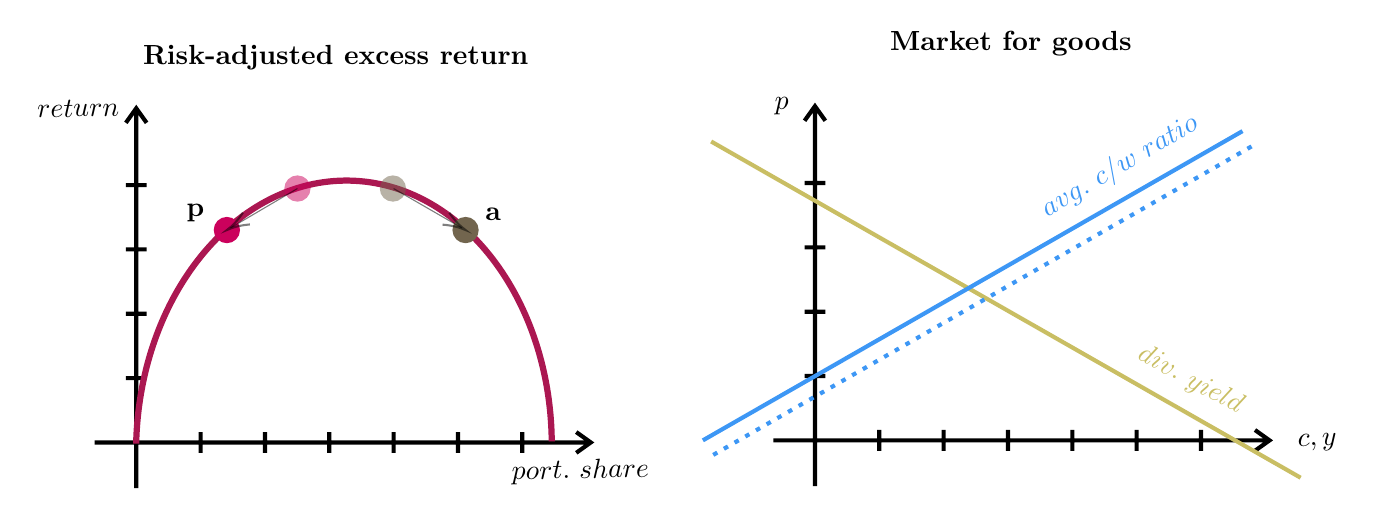
\begin{tikzpicture}[x=0.75pt,y=0.75pt,yscale=-1,xscale=1]
	%uncomment if require: \path (0,235); %set diagram left start at 0, and has height of 235
	
	%Shape: Axis 2D [id:dp8667675453427319] 
	\draw [color={rgb, 255:red, 0; green, 0; blue, 0 }  ,draw opacity=1 ][line width=1.5]  (50,200) -- (289,200)(70,39) -- (70,222) (282,195) -- (289,200) -- (282,205) (65,46) -- (70,39) -- (75,46) (101,195) -- (101,205)(132,195) -- (132,205)(163,195) -- (163,205)(194,195) -- (194,205)(225,195) -- (225,205)(256,195) -- (256,205)(65,169) -- (75,169)(65,138) -- (75,138)(65,107) -- (75,107)(65,76) -- (75,76) ;
	\draw   ;
	%Shape: Arc [id:dp531658316023164] 
	\draw  [draw opacity=0][line width=2.25]  (69.96,200.56) .. controls (71.64,129.28) and (117.82,72.55) .. (173.1,73.85) .. controls (226.88,75.12) and (269.47,130.84) .. (270.19,199.49) -- (170.06,202.92) -- cycle ; \draw  [color={rgb, 255:red, 208; green, 2; blue, 27 }  ,draw opacity=1 ][line width=2.25]  (69.96,200.56) .. controls (71.64,129.28) and (117.82,72.55) .. (173.1,73.85) .. controls (226.88,75.12) and (269.47,130.84) .. (270.19,199.49) ;  
	%Shape: Circle [id:dp05697314227899386] 
	\draw  [draw opacity=0][fill={rgb, 255:red, 248; green, 231; blue, 28 }  ,fill opacity=0.5 ] (141.33,77.67) .. controls (141.33,74.17) and (144.17,71.33) .. (147.67,71.33) .. controls (151.16,71.33) and (154,74.17) .. (154,77.67) .. controls (154,81.16) and (151.16,84) .. (147.67,84) .. controls (144.17,84) and (141.33,81.16) .. (141.33,77.67) -- cycle ;
	%Shape: Circle [id:dp7553623057031522] 
	\draw  [draw opacity=0][fill={rgb, 255:red, 139; green, 87; blue, 42 }  ,fill opacity=0.5 ] (187.33,77.67) .. controls (187.33,74.17) and (190.17,71.33) .. (193.67,71.33) .. controls (197.16,71.33) and (200,74.17) .. (200,77.67) .. controls (200,81.16) and (197.16,84) .. (193.67,84) .. controls (190.17,84) and (187.33,81.16) .. (187.33,77.67) -- cycle ;
	%Shape: Axis 2D [id:dp8452210536537006] 
	\draw [color={rgb, 255:red, 0; green, 0; blue, 0 }  ,draw opacity=1 ][line width=1.5]  (377,199) -- (616,199)(397,38) -- (397,221) (609,194) -- (616,199) -- (609,204) (392,45) -- (397,38) -- (402,45) (428,194) -- (428,204)(459,194) -- (459,204)(490,194) -- (490,204)(521,194) -- (521,204)(552,194) -- (552,204)(583,194) -- (583,204)(392,168) -- (402,168)(392,137) -- (402,137)(392,106) -- (402,106)(392,75) -- (402,75) ;
	\draw   ;
	%Straight Lines [id:da8694501852937826] 
	\draw [color={rgb, 255:red, 245; green, 166; blue, 35 }  ,draw opacity=1 ][line width=1.5]    (347,55) -- (631,217) ;
	%Straight Lines [id:da4872089001830353] 
	\draw [color={rgb, 255:red, 74; green, 144; blue, 226 }  ,draw opacity=1 ][line width=1.5]    (343,199) -- (603,50) ;
	%Shape: Circle [id:dp6153612433225819] 
	\draw  [draw opacity=0][fill={rgb, 255:red, 139; green, 87; blue, 42 }  ,fill opacity=1 ] (222.33,97.67) .. controls (222.33,94.17) and (225.17,91.33) .. (228.67,91.33) .. controls (232.16,91.33) and (235,94.17) .. (235,97.67) .. controls (235,101.16) and (232.16,104) .. (228.67,104) .. controls (225.17,104) and (222.33,101.16) .. (222.33,97.67) -- cycle ;
	%Shape: Circle [id:dp4728310817061825] 
	\draw  [draw opacity=0][fill={rgb, 255:red, 248; green, 231; blue, 28 }  ,fill opacity=1 ] (107.33,97.67) .. controls (107.33,94.17) and (110.17,91.33) .. (113.67,91.33) .. controls (117.16,91.33) and (120,94.17) .. (120,97.67) .. controls (120,101.16) and (117.16,104) .. (113.67,104) .. controls (110.17,104) and (107.33,101.16) .. (107.33,97.67) -- cycle ;
	%Straight Lines [id:da6317730272289139] 
	\draw [color={rgb, 255:red, 0; green, 0; blue, 0 }  ,draw opacity=0.5 ][fill={rgb, 255:red, 0; green, 0; blue, 0 }  ,fill opacity=0 ]   (194,77.67) -- (226.93,96.67) ;
	\draw [shift={(228.67,97.67)}, rotate = 209.98] [color={rgb, 255:red, 0; green, 0; blue, 0 }  ,draw opacity=0.5 ][line width=0.75]    (10.93,-3.29) .. controls (6.95,-1.4) and (3.31,-0.3) .. (0,0) .. controls (3.31,0.3) and (6.95,1.4) .. (10.93,3.29)   ;
	%Straight Lines [id:da22117887446043505] 
	\draw [color={rgb, 255:red, 0; green, 0; blue, 0 }  ,draw opacity=0.5 ][fill={rgb, 255:red, 0; green, 0; blue, 0 }  ,fill opacity=0 ]   (147.67,77.67) -- (115.39,96.65) ;
	\draw [shift={(113.67,97.67)}, rotate = 329.53] [color={rgb, 255:red, 0; green, 0; blue, 0 }  ,draw opacity=0.5 ][line width=0.75]    (10.93,-3.29) .. controls (6.95,-1.4) and (3.31,-0.3) .. (0,0) .. controls (3.31,0.3) and (6.95,1.4) .. (10.93,3.29)   ;
	%Straight Lines [id:da6847983852102553] 
	\draw [color={rgb, 255:red, 74; green, 144; blue, 226 }  ,draw opacity=1 ][line width=1.5]  [dash pattern={on 1.69pt off 2.76pt}]  (348,206) -- (608,57) ;
	
	% Text Node
	\draw (284,214) node  [color={rgb, 255:red, 0; green, 0; blue, 0 }  ,opacity=1 ,rotate=-358.98]  {$port.\ share$};
	% Text Node
	\draw (42,39) node  [color={rgb, 255:red, 0; green, 0; blue, 0 }  ,opacity=1 ,rotate=-358.98]  {$return$};
	% Text Node
	\draw (72,7.43) node [anchor=north west][inner sep=0.75pt]   [align=left] {\textbf{Risk-adjusted excess return}};
	% Text Node
	\draw (544,67) node  [color={rgb, 255:red, 74; green, 144; blue, 226 }  ,opacity=1 ,rotate=-329.57]  {$avg.\ c/w\ ratio$};
	% Text Node
	\draw (639,200) node  [color={rgb, 255:red, 0; green, 0; blue, 0 }  ,opacity=1 ,rotate=-358.98]  {$c,y$};
	% Text Node
	\draw (578,170) node  [color={rgb, 255:red, 245; green, 166; blue, 35 }  ,opacity=1 ,rotate=-28.61]  {$div.\ yield$};
	% Text Node
	\draw (381,38) node  [color={rgb, 255:red, 0; green, 0; blue, 0 }  ,opacity=1 ,rotate=-358.98]  {$p$};
	% Text Node
	\draw (432,0.43) node [anchor=north west][inner sep=0.75pt]   [align=left] {\textbf{Market for goods}};
	% Text Node
	\draw (237,86) node [anchor=north west][inner sep=0.75pt]   [align=left] {\textbf{a}};
	% Text Node
	\draw (93,84) node [anchor=north west][inner sep=0.75pt]   [align=left] {\textbf{p}};
	
	
\end{tikzpicture}
}}

\only<2>{
\scalebox{0.87}{



\tikzset{every picture/.style={line width=0.75pt}} %set default line width to 0.75pt        

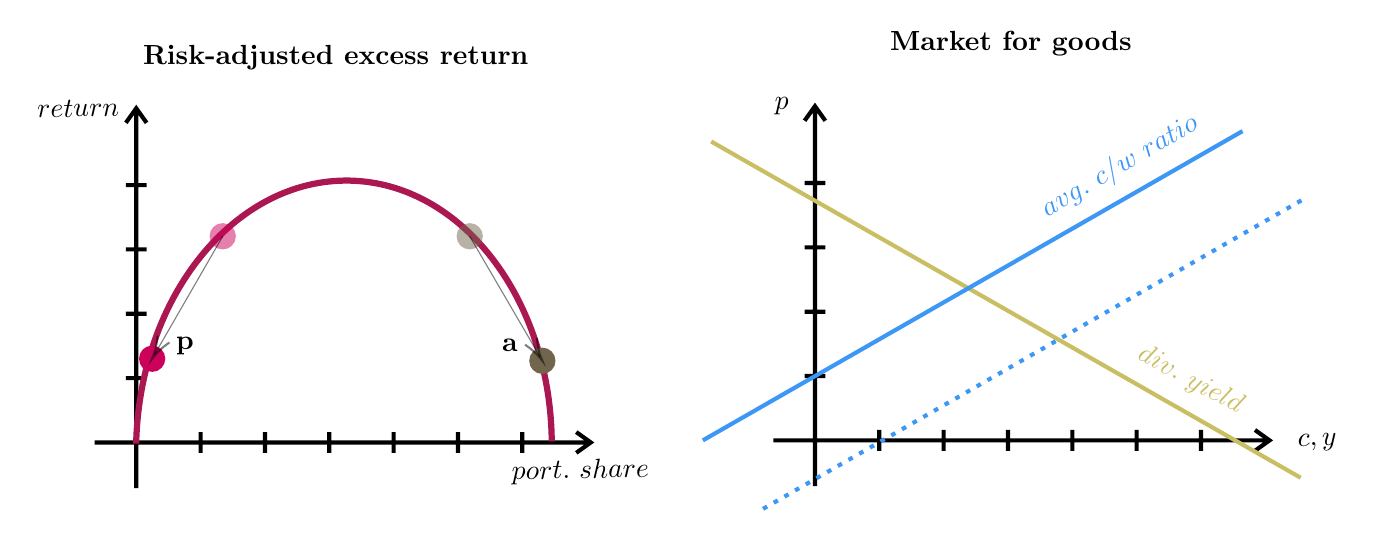
\begin{tikzpicture}[x=0.75pt,y=0.75pt,yscale=-1,xscale=1]
	%uncomment if require: \path (0,235); %set diagram left start at 0, and has height of 235
	
	%Shape: Axis 2D [id:dp17811910341215076] 
	\draw [color={rgb, 255:red, 0; green, 0; blue, 0 }  ,draw opacity=1 ][line width=1.5]  (50,200) -- (289,200)(70,39) -- (70,222) (282,195) -- (289,200) -- (282,205) (65,46) -- (70,39) -- (75,46) (101,195) -- (101,205)(132,195) -- (132,205)(163,195) -- (163,205)(194,195) -- (194,205)(225,195) -- (225,205)(256,195) -- (256,205)(65,169) -- (75,169)(65,138) -- (75,138)(65,107) -- (75,107)(65,76) -- (75,76) ;
	\draw   ;
	%Shape: Arc [id:dp2728896334946356] 
	\draw  [draw opacity=0][line width=2.25]  (69.96,200.56) .. controls (71.64,129.28) and (117.82,72.55) .. (173.1,73.85) .. controls (226.88,75.12) and (269.47,130.84) .. (270.19,199.49) -- (170.06,202.92) -- cycle ; \draw  [color={rgb, 255:red, 208; green, 2; blue, 27 }  ,draw opacity=1 ][line width=2.25]  (69.96,200.56) .. controls (71.64,129.28) and (117.82,72.55) .. (173.1,73.85) .. controls (226.88,75.12) and (269.47,130.84) .. (270.19,199.49) ;  
	%Shape: Circle [id:dp09152732788574003] 
	\draw  [draw opacity=0][fill={rgb, 255:red, 248; green, 231; blue, 28 }  ,fill opacity=0.5 ] (105.33,100.67) .. controls (105.33,97.17) and (108.17,94.33) .. (111.67,94.33) .. controls (115.16,94.33) and (118,97.17) .. (118,100.67) .. controls (118,104.16) and (115.16,107) .. (111.67,107) .. controls (108.17,107) and (105.33,104.16) .. (105.33,100.67) -- cycle ;
	%Shape: Circle [id:dp8702384042700901] 
	\draw  [draw opacity=0][fill={rgb, 255:red, 139; green, 87; blue, 42 }  ,fill opacity=0.5 ] (224.33,100.67) .. controls (224.33,97.17) and (227.17,94.33) .. (230.67,94.33) .. controls (234.16,94.33) and (237,97.17) .. (237,100.67) .. controls (237,104.16) and (234.16,107) .. (230.67,107) .. controls (227.17,107) and (224.33,104.16) .. (224.33,100.67) -- cycle ;
	%Shape: Axis 2D [id:dp6014255008545599] 
	\draw [color={rgb, 255:red, 0; green, 0; blue, 0 }  ,draw opacity=1 ][line width=1.5]  (377,199) -- (616,199)(397,38) -- (397,221) (609,194) -- (616,199) -- (609,204) (392,45) -- (397,38) -- (402,45) (428,194) -- (428,204)(459,194) -- (459,204)(490,194) -- (490,204)(521,194) -- (521,204)(552,194) -- (552,204)(583,194) -- (583,204)(392,168) -- (402,168)(392,137) -- (402,137)(392,106) -- (402,106)(392,75) -- (402,75) ;
	\draw   ;
	%Straight Lines [id:da943055555850097] 
	\draw [color={rgb, 255:red, 245; green, 166; blue, 35 }  ,draw opacity=1 ][line width=1.5]    (347,55) -- (631,217) ;
	%Straight Lines [id:da12202983705810633] 
	\draw [color={rgb, 255:red, 74; green, 144; blue, 226 }  ,draw opacity=1 ][line width=1.5]    (343,199) -- (603,50) ;
	%Shape: Circle [id:dp9185533411503766] 
	\draw  [draw opacity=0][fill={rgb, 255:red, 139; green, 87; blue, 42 }  ,fill opacity=1 ] (259.33,160.67) .. controls (259.33,157.17) and (262.17,154.33) .. (265.67,154.33) .. controls (269.16,154.33) and (272,157.17) .. (272,160.67) .. controls (272,164.16) and (269.16,167) .. (265.67,167) .. controls (262.17,167) and (259.33,164.16) .. (259.33,160.67) -- cycle ;
	%Shape: Circle [id:dp458319980377794] 
	\draw  [draw opacity=0][fill={rgb, 255:red, 248; green, 231; blue, 28 }  ,fill opacity=1 ] (71.33,159.67) .. controls (71.33,156.17) and (74.17,153.33) .. (77.67,153.33) .. controls (81.16,153.33) and (84,156.17) .. (84,159.67) .. controls (84,163.16) and (81.16,166) .. (77.67,166) .. controls (74.17,166) and (71.33,163.16) .. (71.33,159.67) -- cycle ;
	%Straight Lines [id:da5461592683560248] 
	\draw [color={rgb, 255:red, 0; green, 0; blue, 0 }  ,draw opacity=0.5 ][fill={rgb, 255:red, 0; green, 0; blue, 0 }  ,fill opacity=0 ]   (230.67,100.67) -- (264.66,158.94) ;
	\draw [shift={(265.67,160.67)}, rotate = 239.74] [color={rgb, 255:red, 0; green, 0; blue, 0 }  ,draw opacity=0.5 ][line width=0.75]    (10.93,-3.29) .. controls (6.95,-1.4) and (3.31,-0.3) .. (0,0) .. controls (3.31,0.3) and (6.95,1.4) .. (10.93,3.29)   ;
	%Straight Lines [id:da04864508639252052] 
	\draw [color={rgb, 255:red, 0; green, 0; blue, 0 }  ,draw opacity=0.5 ][fill={rgb, 255:red, 0; green, 0; blue, 0 }  ,fill opacity=0 ]   (111.67,100.67) -- (78.67,157.93) ;
	\draw [shift={(77.67,159.67)}, rotate = 299.95] [color={rgb, 255:red, 0; green, 0; blue, 0 }  ,draw opacity=0.5 ][line width=0.75]    (10.93,-3.29) .. controls (6.95,-1.4) and (3.31,-0.3) .. (0,0) .. controls (3.31,0.3) and (6.95,1.4) .. (10.93,3.29)   ;
	%Straight Lines [id:da7145890387073353] 
	\draw [color={rgb, 255:red, 74; green, 144; blue, 226 }  ,draw opacity=1 ][line width=1.5]  [dash pattern={on 1.69pt off 2.76pt}]  (372,232) -- (632,83) ;
	
	% Text Node
	\draw (284,214) node  [color={rgb, 255:red, 0; green, 0; blue, 0 }  ,opacity=1 ,rotate=-358.98]  {$port.\ share$};
	% Text Node
	\draw (42,39) node  [color={rgb, 255:red, 0; green, 0; blue, 0 }  ,opacity=1 ,rotate=-358.98]  {$return$};
	% Text Node
	\draw (72,7.43) node [anchor=north west][inner sep=0.75pt]   [align=left] {\textbf{Risk-adjusted excess return}};
	% Text Node
	\draw (544,67) node  [color={rgb, 255:red, 74; green, 144; blue, 226 }  ,opacity=1 ,rotate=-329.57]  {$avg.\ c/w\ ratio$};
	% Text Node
	\draw (639,200) node  [color={rgb, 255:red, 0; green, 0; blue, 0 }  ,opacity=1 ,rotate=-358.98]  {$c,y$};
	% Text Node
	\draw (578,170) node  [color={rgb, 255:red, 245; green, 166; blue, 35 }  ,opacity=1 ,rotate=-28.61]  {$div.\ yield$};
	% Text Node
	\draw (381,38) node  [color={rgb, 255:red, 0; green, 0; blue, 0 }  ,opacity=1 ,rotate=-358.98]  {$p$};
	% Text Node
	\draw (432,0.43) node [anchor=north west][inner sep=0.75pt]   [align=left] {\textbf{Market for goods}};
	% Text Node
	\draw (245,149) node [anchor=north west][inner sep=0.75pt]   [align=left] {\textbf{a}};
	% Text Node
	\draw (88,148) node [anchor=north west][inner sep=0.75pt]   [align=left] {\textbf{p}};
	
	
\end{tikzpicture}
}
}
\end{frame}

\begin{frame}{Market Elasticity}
    \begin{prop}[Aggregate market  elasticity]\label{prop:elasticity_passive_demand}
    	The inverse aggregate market elasticity, $ 1/\varepsilon_M $, is given by:
    	\begin{equation*}
    		\varepsilon_{M}^{-1}=%\frac{1}{p(X, \epsilon)} \frac{\partial p(X, \epsilon)}{\partial F(X, \epsilon)}=
    		\left(1-\psi^{-1}\right) \frac{\gamma \sigma^{2}}{y^*} \textcolor{red}{\frac{\overline{\alpha}_{p,t}^{optimal}-\overline{\alpha}_{p}}{1-x_{0}-x_c} (1-x_c)}+\mathcal{O}\left(\epsilon^{2}\right),
    	\end{equation*}		
    where $\overline{\alpha}_{p,t}^{optimal}$ is the optimal portfolio weight for passive investors.
    % 	where $ x_{a} \equiv 1-x_{0} $ denotes the wealth share of active investors.
    \end{prop}
\end{frame}

\begin{frame}{The dynamics of the portfolio gap}
	\begin{wideitemize}
		\item The (privately) optimal portfolio:
\begin{equation}
	\overline{\alpha}_{p,t}^{optimal} = 1 -\textcolor{red}{\frac{x_u}{1-x_c}}\frac{\gamma_0-\mathbb{E}^u[\gamma_j] }{\gamma} - \frac{x_c(\frac{\overline{\sigma}}{\|\sigma\|}-1)  }{1-x_c}.\nonumber
\end{equation}
\vspM
\item Active investors lose wealth in bad times
\begin{itemize}
	\item Passive investors should invest more in the stock market
	\item But they typically move funds out in bad times
\end{itemize}
	\end{wideitemize}
	
	
\end{frame}


\begin{frame}{Inverse market elasticity: passive demand}
    \centering
    
\includegraphics[width=0.75\textwidth]{figures/elasticity_passive.pdf}
    % \resizebox{0.5\textwidth}{!}{\begin{tikzpicture}[/tikz/background rectangle/.style={fill={rgb,1:red,1.0;green,1.0;blue,1.0}, draw opacity={1.0}}, show background rectangle]
\begin{axis}[point meta max={nan}, point meta min={nan}, title={Price Impact (passive demand)}, title style={at={{(0.5,1)}}, anchor={south}, font={{\fontsize{14 pt}{18.2 pt}\selectfont}}, color={rgb,1:red,0.0;green,0.0;blue,0.0}, draw opacity={1.0}, rotate={0.0}}, legend style={color={rgb,1:red,0.0;green,0.0;blue,0.0}, draw opacity={0.0}, line width={1}, solid, fill={rgb,1:red,0.0;green,0.0;blue,0.0}, fill opacity={0.0}, text opacity={1.0}, font={{\fontsize{8 pt}{10.4 pt}\selectfont}}, text={rgb,1:red,0.0;green,0.0;blue,0.0}, cells={anchor={center}}, at={(0.98, 0.98)}, anchor={north east}}, axis background/.style={fill={rgb,1:red,1.0;green,1.0;blue,1.0}, opacity={1.0}}, anchor={north west}, xshift={1.0mm}, yshift={-1.0mm}, width={150.4mm}, height={99.6mm}, scaled x ticks={false}, xlabel={$x_a$}, x tick style={color={rgb,1:red,0.0;green,0.0;blue,0.0}, opacity={1.0}}, x tick label style={color={rgb,1:red,0.0;green,0.0;blue,0.0}, opacity={1.0}, rotate={0}}, xlabel style={at={(ticklabel cs:0.5)}, anchor=near ticklabel, at={{(ticklabel cs:0.5)}}, anchor={near ticklabel}, font={{\fontsize{11 pt}{14.3 pt}\selectfont}}, color={rgb,1:red,0.0;green,0.0;blue,0.0}, draw opacity={1.0}, rotate={0.0}}, xmajorgrids={true}, xmin={-0.004699999999999999}, xmax={0.5147}, xtick={{0.0,0.1,0.2,0.30000000000000004,0.4,0.5}}, xticklabels={{$0.0$,$0.1$,$0.2$,$0.3$,$0.4$,$0.5$}}, xtick align={inside}, xticklabel style={font={{\fontsize{8 pt}{10.4 pt}\selectfont}}, color={rgb,1:red,0.0;green,0.0;blue,0.0}, draw opacity={1.0}, rotate={0.0}}, x grid style={color={rgb,1:red,0.0;green,0.0;blue,0.0}, draw opacity={0.1}, line width={0.5}, solid}, axis x line*={left}, x axis line style={color={rgb,1:red,0.0;green,0.0;blue,0.0}, draw opacity={1.0}, line width={1}, solid}, scaled y ticks={false}, ylabel={$\varepsilon_M^{-1}$}, y tick style={color={rgb,1:red,0.0;green,0.0;blue,0.0}, opacity={1.0}}, y tick label style={color={rgb,1:red,0.0;green,0.0;blue,0.0}, opacity={1.0}, rotate={0}}, ylabel style={at={(ticklabel cs:0.5)}, anchor=near ticklabel, at={{(ticklabel cs:0.5)}}, anchor={near ticklabel}, font={{\fontsize{11 pt}{14.3 pt}\selectfont}}, color={rgb,1:red,0.0;green,0.0;blue,0.0}, draw opacity={1.0}, rotate={0.0}}, ymajorgrids={true}, ymin={-0.6043165467625898}, ymax={20.74820143884892}, ytick={{0.0,5.0,10.0,15.0,20.0}}, yticklabels={{$0$,$5$,$10$,$15$,$20$}}, ytick align={inside}, yticklabel style={font={{\fontsize{8 pt}{10.4 pt}\selectfont}}, color={rgb,1:red,0.0;green,0.0;blue,0.0}, draw opacity={1.0}, rotate={0.0}}, y grid style={color={rgb,1:red,0.0;green,0.0;blue,0.0}, draw opacity={0.1}, line width={0.5}, solid}, axis y line*={left}, y axis line style={color={rgb,1:red,0.0;green,0.0;blue,0.0}, draw opacity={1.0}, line width={1}, solid}, colorbar={false}]
    \addplot[color={rgb,1:red,0.0;green,0.6056;blue,0.9787}, name path={f4cdcfa1-7372-4f0e-b9fa-f7a37af4e78c}, draw opacity={1.0}, line width={1.5}, dashed]
        table[row sep={\\}]
        {
            \\
            0.01  20.14388489208633  \\
            0.02  10.071942446043165  \\
            0.03  6.71462829736211  \\
            0.04  5.0359712230215825  \\
            0.05  4.028776978417266  \\
            0.06  3.357314148681055  \\
            0.07  2.877697841726618  \\
            0.08  2.5179856115107913  \\
            0.09  2.238209432454037  \\
            0.1  2.014388489208633  \\
            0.11  1.831262262916939  \\
            0.12  1.6786570743405276  \\
            0.13  1.549529607083564  \\
            0.14  1.438848920863309  \\
            0.15  1.3429256594724222  \\
            0.16  1.2589928057553956  \\
            0.17  1.184934405416843  \\
            0.18  1.1191047162270185  \\
            0.19  1.0602044680045437  \\
            0.2  1.0071942446043165  \\
            0.21  0.9592326139088729  \\
            0.22  0.9156311314584695  \\
            0.23  0.8758210822646231  \\
            0.24  0.8393285371702638  \\
            0.25  0.8057553956834532  \\
            0.26  0.774764803541782  \\
            0.27  0.7460698108180122  \\
            0.28  0.7194244604316545  \\
            0.29  0.6946167204167701  \\
            0.3  0.6714628297362111  \\
            0.31  0.6498027384543978  \\
            0.32  0.6294964028776978  \\
            0.33  0.6104207543056464  \\
            0.34  0.5924672027084215  \\
            0.35  0.5755395683453238  \\
            0.36  0.5595523581135092  \\
            0.37  0.5444293214077387  \\
            0.38  0.5301022340022719  \\
            0.39  0.5165098690278547  \\
            0.4  0.5035971223021583  \\
            0.41  0.49131426566064224  \\
            0.42  0.47961630695443647  \\
            0.43  0.4684624393508449  \\
            0.44  0.45781556572923476  \\
            0.45  0.44764188649080733  \\
            0.46  0.43791054113231154  \\
            0.47  0.42859329557630493  \\
            0.48  0.4196642685851319  \\
            0.49  0.41109969167523125  \\
            0.5  0.4028776978417266  \\
        }
        ;
    \addlegendentry {$\overline{\alpha}_p=0.00$}
    \addplot[color={rgb,1:red,0.8889;green,0.4356;blue,0.2781}, name path={ac2c085b-b6ea-4b31-af2b-7202cf3d5eb3}, draw opacity={1.0}, line width={1.5}, solid]
        table[row sep={\\}]
        {
            \\
            0.01  15.107913669064747  \\
            0.02  7.553956834532373  \\
            0.03  5.0359712230215825  \\
            0.04  3.7769784172661867  \\
            0.05  3.0215827338129495  \\
            0.06  2.5179856115107913  \\
            0.07  2.158273381294964  \\
            0.08  1.8884892086330933  \\
            0.09  1.6786570743405276  \\
            0.1  1.5107913669064748  \\
            0.11  1.3734466971877044  \\
            0.12  1.2589928057553956  \\
            0.13  1.162147205312673  \\
            0.14  1.079136690647482  \\
            0.15  1.0071942446043167  \\
            0.16  0.9442446043165467  \\
            0.17  0.8887008040626322  \\
            0.18  0.8393285371702638  \\
            0.19  0.7951533510034078  \\
            0.2  0.7553956834532374  \\
            0.21  0.7194244604316548  \\
            0.22  0.6867233485938522  \\
            0.23  0.6568658116984673  \\
            0.24  0.6294964028776978  \\
            0.25  0.60431654676259  \\
            0.26  0.5810736026563365  \\
            0.27  0.5595523581135091  \\
            0.28  0.539568345323741  \\
            0.29  0.5209625403125776  \\
            0.3  0.5035971223021584  \\
            0.31  0.4873520538407984  \\
            0.32  0.47212230215827333  \\
            0.33  0.45781556572923476  \\
            0.34  0.4443504020313161  \\
            0.35  0.43165467625899284  \\
            0.36  0.4196642685851319  \\
            0.37  0.408321991055804  \\
            0.38  0.3975766755017039  \\
            0.39  0.387382401770891  \\
            0.4  0.3776978417266187  \\
            0.41  0.3684856992454817  \\
            0.42  0.3597122302158274  \\
            0.43  0.35134682951313373  \\
            0.44  0.3433616742969261  \\
            0.45  0.3357314148681055  \\
            0.46  0.3284329058492336  \\
            0.47  0.3214449716822287  \\
            0.48  0.3147482014388489  \\
            0.49  0.30832476875642345  \\
            0.5  0.302158273381295  \\
        }
        ;
    \addlegendentry {$\overline{\alpha}_p=0.25$}
    \addplot[color={rgb,1:red,0.2422;green,0.6433;blue,0.3044}, name path={5773374e-7c29-4047-9b85-4c25a864e67f}, draw opacity={1.0}, line width={1.5}, dashdotted]
        table[row sep={\\}]
        {
            \\
            0.01  10.071942446043165  \\
            0.02  5.0359712230215825  \\
            0.03  3.357314148681055  \\
            0.04  2.5179856115107913  \\
            0.05  2.014388489208633  \\
            0.06  1.6786570743405276  \\
            0.07  1.438848920863309  \\
            0.08  1.2589928057553956  \\
            0.09  1.1191047162270185  \\
            0.1  1.0071942446043165  \\
            0.11  0.9156311314584695  \\
            0.12  0.8393285371702638  \\
            0.13  0.774764803541782  \\
            0.14  0.7194244604316545  \\
            0.15  0.6714628297362111  \\
            0.16  0.6294964028776978  \\
            0.17  0.5924672027084215  \\
            0.18  0.5595523581135092  \\
            0.19  0.5301022340022719  \\
            0.2  0.5035971223021583  \\
            0.21  0.47961630695443647  \\
            0.22  0.45781556572923476  \\
            0.23  0.43791054113231154  \\
            0.24  0.4196642685851319  \\
            0.25  0.4028776978417266  \\
            0.26  0.387382401770891  \\
            0.27  0.3730349054090061  \\
            0.28  0.35971223021582727  \\
            0.29  0.34730836020838507  \\
            0.3  0.33573141486810554  \\
            0.31  0.3249013692271989  \\
            0.32  0.3147482014388489  \\
            0.33  0.3052103771528232  \\
            0.34  0.29623360135421073  \\
            0.35  0.2877697841726619  \\
            0.36  0.2797761790567546  \\
            0.37  0.27221466070386935  \\
            0.38  0.2650511170011359  \\
            0.39  0.25825493451392734  \\
            0.4  0.2517985611510791  \\
            0.41  0.24565713283032112  \\
            0.42  0.23980815347721823  \\
            0.43  0.23423121967542246  \\
            0.44  0.22890778286461738  \\
            0.45  0.22382094324540366  \\
            0.46  0.21895527056615577  \\
            0.47  0.21429664778815247  \\
            0.48  0.20983213429256595  \\
            0.49  0.20554984583761562  \\
            0.5  0.2014388489208633  \\
        }
        ;
    \addlegendentry {$\overline{\alpha}_p=0.50$}
    \addplot[color={rgb,1:red,0.7644;green,0.4441;blue,0.8243}, name path={360eb9b8-2ddc-4974-8108-fe0426cc3372}, draw opacity={1.0}, line width={1.5}, dashed]
        table[row sep={\\}]
        {
            \\
            0.01  0.0  \\
            0.02  0.0  \\
            0.03  0.0  \\
            0.04  0.0  \\
            0.05  0.0  \\
            0.06  0.0  \\
            0.07  0.0  \\
            0.08  0.0  \\
            0.09  0.0  \\
            0.1  0.0  \\
            0.11  0.0  \\
            0.12  0.0  \\
            0.13  0.0  \\
            0.14  0.0  \\
            0.15  0.0  \\
            0.16  0.0  \\
            0.17  0.0  \\
            0.18  0.0  \\
            0.19  0.0  \\
            0.2  0.0  \\
            0.21  0.0  \\
            0.22  0.0  \\
            0.23  0.0  \\
            0.24  0.0  \\
            0.25  0.0  \\
            0.26  0.0  \\
            0.27  0.0  \\
            0.28  0.0  \\
            0.29  0.0  \\
            0.3  0.0  \\
            0.31  0.0  \\
            0.32  0.0  \\
            0.33  0.0  \\
            0.34  0.0  \\
            0.35  0.0  \\
            0.36  0.0  \\
            0.37  0.0  \\
            0.38  0.0  \\
            0.39  0.0  \\
            0.4  0.0  \\
            0.41  0.0  \\
            0.42  0.0  \\
            0.43  0.0  \\
            0.44  0.0  \\
            0.45  0.0  \\
            0.46  0.0  \\
            0.47  0.0  \\
            0.48  0.0  \\
            0.49  0.0  \\
            0.5  0.0  \\
        }
        ;
    \addlegendentry {$\overline{\alpha}_p=1.00$}
\end{axis}
\end{tikzpicture}
} 
\end{frame}

\begin{frame}{Inverse market elasticity: preference heterogeneity}
    \centering
    
\includegraphics[width=\textwidth]{figures/elasticity_heterog.pdf}
\end{frame}

\begin{frame}{Market elasticity and volatility}
	\centering
	\includegraphics[width=0.65\textwidth]{figures/vol.pdf}
	\[
	\sigma_{p,t} = \frac{p_x(X_t)}{p(X_t)} \sigma_{x,t} + \frac{p_{\overline{\alpha}_p}(X_t)}{p(X_t)} \sigma_p \sqrt{\overline{\alpha}_p}
	\]
\end{frame}

%\begin{frame}{State space: ergodic distribution}
%	\centering
%	
\includegraphics[width=\textwidth]{figures/state_space_ergodic.pdf}
%\end{frame}

%\begin{frame}{Next steps}
%    \begin{wideitemize}
%        %\item Bring back the flow shocks and quantitatively evaluate its importance
%        % \begin{itemize}
%        %     \item 
%        % \end{itemize}
%        \item Calibrate the model to the Flow of Funds with multiple sectors
%        \begin{itemize}
%            \item rich heterogeneity in the model is key to match the data\vspM
%            \item challenging: solving and estimating a high-dim. macro-finance model
%        \end{itemize}
%        \item Can frictions generate observed levels of market volatility?
%        \begin{itemize}
%            \item flow volatility\vspM
%            \item high price impact?
%        \end{itemize}
%    \end{wideitemize}
%\end{frame}

\begin{frame}{Conclusion}
	\begin{itemize}
		\item Macro elasticity in a GE framework with rich heterogeneity and frictions\vspM
		\begin{itemize}
			\item passive demand \& leverage-constrained active investors\vspM
		\end{itemize}
		\item No macro price impact \vspM
		\begin{itemize}
			\item in frictionless settings\vspM
			\item when risk is perfectly shared\vspM
		\end{itemize}
		%\item Aggregate elasticity is state-dependent
		\item Excess volatility from flow shocks and inelastic markets\vspM
		\item Next steps\vspM
		\begin{itemize}
			\item use 13F holdings data to calibrate the model\vspM
			\item which sectors to consider?\vspM
			\item excess volatility puzzle
		\end{itemize}
	\end{itemize}
\end{frame}
{
	\setbeamercolor{background canvas}{bg=mDarkTeal}
	\begin{frame}[plain,noframenumbering]
		\begin{center}
			\huge \textcolor{white}{\textbf{Thank you!}}
		\end{center}
	\end{frame}

	
}

\end{document}
